\documentclass[12 pt]{article}
\usepackage{hyperref, fancyhdr, setspace, enumerate, amsmath,
  lastpage, amssymb, algpseudocode, tikz, listings,
  marvosym, stmaryrd, collectbox, wasysym, algorithm}
\usetikzlibrary{shapes.geometric}
\usetikzlibrary{positioning,chains,fit,shapes,calc,arrows.meta,matrix,automata}
\usepackage[margin=1 in]{geometry}
\allowdisplaybreaks
% \usepackage[dvipsnames]{xcolor}   %May be necessary if you want to color links
\hypersetup{
  % colorlinks=true, %set true if you want colored links
  linktoc=all,     %set to all if you want both sections and subsections linked
  linkcolor=black,  %choose some color if you want links to stand out
}
% New environment to scale prooftrees, from https://tex.stackexchange.com/questions/104554/how-to-scale-prooftree-environment-bussproofs-package
\newenvironment{scprooftree}[1]%
  {\gdef\scalefactor{#1}\begin{center}\proofSkipAmount \leavevmode}%
  {\scalebox{\scalefactor}{\DisplayProof}\proofSkipAmount \end{center}
}
%New command \mybox to box something
\newcommand{\mybox}{%
\collectbox{%
	\setlength{\fboxsep}{3pt}%
	\fbox{\BOXCONTENT}%
	}%
}

\usepackage{graphicx}
\graphicspath{{Images/}}
\author{Julian Lore}
\date{Last updated: \today}
\title{COMP 330: Theory of Computation}
\pagestyle{fancy}
\lhead{COMP 330}
\chead{\leftmark}
\rhead{Julian Lore}
\cfoot{Page \thepage \ of \pageref{LastPage}}
\newcommand{\tab}[1]{\hspace{.2\textwidth}\rlap{#1}}
\newenvironment{rcases}
  {\left.\begin{aligned}}
  {\end{aligned}\right\rbrace}
\begin{document}
\onehalfspacing
\maketitle
\tableofcontents
\section{09/03/19}
\paragraph{Language}
Let $\Sigma$ be a finite alphabet (set). Let $\Sigma^*$ be all possible
sequences of elements from alphabet (infinitely many sequences). A
\textbf{language} $L$ is any subset of $\Sigma^*$. It will tell you for
every possible string whether it is in $L$ or not. An algorithm $A$
decides a language $L$ if it can say whether $x\in L$ or $x\notin L$
(can answer yes or no).

Example: alphabet is $\{0,1\}$. Our language can be all prime numbers
represented as binary numbers. We can then make an algorithm that
decides if a binary string $x$ is a prime or not (i.e.\ is it in our language?).

Generally however, we will ask ourselves, if we can define a language,
can we come up with an algorithm to decide it?

$$\text{All languages} \supset \text{Languages we can describe}
\supset \text{Languages that are decidable}$$
\begin{itemize}
\item $|\text{All languages}| = \mathbb{R}$
\item $|\text{Languages we can describe}| = \mathbb{N}$
\item $|\text{Languages we can decide}| = \mathbb{N}$ (however it is
  much smaller than what we can describe). Clearly things that are
  decidable are describable, as the algorithm to decide it can also
  describe it.
\end{itemize}
\paragraph{Post Correspondence Problem} \label{pcp}You are given a set of tiles
that have strings.
\\
\begin{tabular}{|c| c| c| c| c |c|}
  \hline aaa&a&bbb&aa&&b
  \\ bb & bb & a & a & bb &
  \\ \hline
\end{tabular}
\\ Is there a sequence of these tiles that the concatenation of the
top string is the same as the bottom string?
% \\ Solution for our example:
% \\
% \begin{tabular}{|c| c| c| c| c |c|}
%   \hline aa&a&bbb&aa&&b
%   \\ bb & bb & a & a & bb &
                              %     \\ \hline
% \end{tabular}
\\ The general version of the problem is $n$ tiles, $u_1/v_1 \ldots
u_n/v_n$ where each $u_i$ and $v_i$ are sequences of letters. Is there
a $k$ and a sequence $\langle i_1, i_2, \ldots, i_k \rangle$ ($1 \leq
i_j \leq n, \forall j \in \{1,\ldots,n\}$), such that $u_{i_1} \ldots
u_{i_k} = v_{i_1} \ldots v_{i_k}$.
\paragraph{Theorem} The Post Correspondence Problem cannot be decided by any
algorithm/computer program. No algorithm can give a no answer in a
finite amount of time. We can, however, give yes answers/find a
solution if one exists.
\section{09/05/19}
To prove the theorem, we use a reduction technique. If PCP was
decidable then another undecidable problem, the halting problem, would
also be decidable. We will often reduce problems to others in this
course.
\paragraph{The Halting Problem}
Note that an algorithm is just text. An algorithm can receives text as
input and thus can receive the text of an algorithm as input.

So the Halting Problem is as follows: Given two texts $A$ and $B$, $A$
being an algorithm, $B$ being an input. Will $A$ halt (instead of loop
forever) on input $B$?

Back to PCP, any algorithm that can decide PCP can be converted to an
algorithm to decide the Halting Problem. Thus we conclude that PCP
cannot be decided.

\paragraph{Computability Theory}
Consists of the ability to distinguish between all languages,
describable languages and decidable languages, the difference between
describable and decidable languages being the most important.
\paragraph{Complexity Theory} Distinguishing between languages we can
decide, languages we can check efficiently and languages we can decide
efficiently (polynomial).
\paragraph{Example} Map coloring, can we color a map such that all the
neighbors have different colors? Without a color restriction, we can
just use different colors for each area. How about with 2 colors? This
is the 2-coloring problem. This can easily be checked, an area cannot
have two neighbors that are also neighbors. Or we can just try
coloring the map with two colors and see if we get a conflict.

How about 3 colors? Try coloring the map. But when trying to color,
when we reach a neighbor, we have a choice between either of the two
remaining colors. So naturally we should try both. Then checking this
becomes exponential.

Note that checking the validity of an $n$-coloring is much simpler
than finding said $n$-coloring. Finding is exponential, but checking
just requires verifying the neighbors and is polynomial.

\paragraph{Summary of $K$-coloring of maps}
\begin{itemize}
\item $K = 1$, can only color maps with zero or one region.
\item $K = 2$, impossible when three regions are all neighbors,
  otherwise valid. Easy to decide.
\item $K = 3$, no known efficient algorithm to decide, easy to check. $NP$-complete.
\item $K \geq 4$, all maps are $K$-colorable (there exists a long
  proof for $4$, people managed to reduce the infinite cases of maps
  to about $300,000$ cases that were checked). Not easy to find, easy
  to verify.
\end{itemize}
$3$-coloring of maps is a special type of problem (NP-complete
problems), as solving this efficiently would solve many other problems
efficiently.
\paragraph{Examples of NP-Complete Problems}
\begin{itemize}
\item SAT:\ given a boolean formula (logic formula), does there exist
  a truth assignment such that the formula is true?
\item Traveling Salesman:\ given a set of cities and distances between
  them, find the shortest path to visit each city once.
\item Knapsack:\ given items with weights, is there a subset of them
  of weight $K$?
\end{itemize}
Many practical problems are NP-Complete. If we can solve one
efficiently, they can all be solved efficiently. In practice, some
special cases of the problems can be solved efficiently.
\paragraph{Tractable Problems (P)} Problems for which we can
efficiently (polynomial) decide whether an instance of a problem is a
yes or no, i.e.\ is this map $2$-colorable?
\\ Examples:
\begin{itemize}
\item $2$-colorability of maps
\item Primality testing
\item Solving $N \times N \times N$ Rubik's cubes
\item Finding a word in a dictionary
\item Sorting
\end{itemize}
$P$ stands for Polynomial-Time computable. Sometimes problems may be
efficiently solvable but it might not be provable.

Back to complexity theory, $\text{Decidable languages} \supset NP
\supset P$. NP-Complete problems are a subset of NP problems. If we
can bring the complete problems to P, then $NP = P$. We tend to
believe $P \neq NP$ as all attempts to show they're equal so far have
failed.

\paragraph{PSpace Completeness} problems that require polynomial space to be solved but can
still take very long. Again, if any of these problems can be done in
polynomial time, then they can all be solved in polynomial time.
\\ Example: Geography game. This is a two player game. Given a set of
country names, the first player chooses a country, then the other
player must choose a country whose name starts with the last letter of
the country chosen by the previous player. Someone wins if their
opponent cannot choose a country.
\\ Generalized geography game consists of an arbitrary set of names
$w_1, \ldots, w_n$ instead. Is there a winning strategy for the
starting player? Intuitively, you can solve this by enumerating all
possibilities. You won't be able to use more than $n$ names, but you
may have to enumerate many possibilities. So you can check all
possibilities without using much space (polynomial).

PSpace is a superset of NP (although we don't know if they're unequal
or not), which also has a complete subset.

\paragraph{Theoretical Computer Science}
Want to find efficient solutions to many problems, this is the
algorithm and data structures part.

We also want to prove that some problems are not computable within a
certain time or space.

We also consider new models of computation (like quantum
computers). This won't disrupt our notion of computability (whether
something can be computed) but it will disrupt our notion of
complexity, as lots of things will be faster/easier to compute.

\subsection{Deterministic Finite Automata and Regular Expressions}
DFAs consists of labeled nodes (states corresponding to the memory of
a device, the device only knows what state it is in) with edges
between them, allowing the device to move from one state to another
depending on the input (edges are labeled).

\paragraph{Examples of DFAs}
\begin{itemize}
\item Swing doors (before motion detectors) had a front pad and a rear
  pad.

  It would have a closed state and an open state. In the closed state,
  if someone is on the front pad and no one is on the rear pad, the
  door would go to the open state until no one is on either pad. If in
  the closed state but someone is on the rear pad, it should never
  open. We can draw a DFA for this.
\end{itemize}
\section{09/10/19}
\paragraph{DFA} A finite automaton is a 5-tuple $(Q, \Sigma, \delta,
q_0, F)$ where:
\begin{itemize}
\item $Q$: States
\item $\Sigma$: Alphabet (fixed string inputs it can take)
\item $\delta: Q \times \Sigma \to Q$: Transition function (how you should go from a certain state to
  another if your next symbol is something from the alphabet, read
  symbols one by one), displayed by arrows from state to state. For
  the simple module, we assume every state has a transition state for
  every symbol of the alphabet. We can describe $\delta$ either via a
  picture of the DFA or with a table.
\item $q_0 \in Q$: Start state. Indicated by an incoming arrow from nowhere. There
  is only one start state in a DFA as it is deterministic.
\item $F \subseteq Q$: Accept states. There can be multiple accept states, identified
  by an extra circle in the node. If you reach the end of the string
  and are in an accept state, the automaton will accept the string,
  otherwise it will reject it.

  If $F = Q$, then all strings will be accepted, i.e.\ the language is $\Sigma^*$.
\end{itemize}
Note that the empty string is a valid input. It will only be accepted
if the start state is an accept state.
\paragraph{Ex}~\\
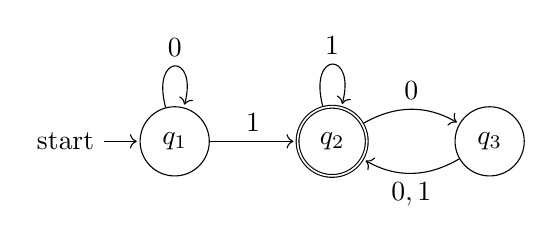
\begin{tikzpicture}[shorten >=1pt,node distance=2 cm,on grid,auto]
  \node[state,initial] (q_1)   {$q_1$};
  \node[state,accepting](q_2) [right=of q_1] {$q_2$};
  \node[state](q_3) [right=of q_2] {$q_3$};
  \path[->]
  (q_1) edge [loop above] node {$0$} ()
  (q_1) edge node {$1$} (q_2)
  (q_2) edge [loop above] node {$1$} ()
  (q_2) edge [bend left] node {$0$} (q_3)
  (q_3) edge [bend left] node {$0,1$} (q_2)
  ;
\end{tikzpicture}
\begin{itemize}
\item $Q = \left\{q_1, q_2, q_3\right\}$
\item $\Sigma = \left\{0,1\right\}$
\item $\delta = $
  \begin{tabular}{c | c c}
    &$0$&$1$
    \\ \hline $q_1$ & $q_1$ & $q_2$
    \\ $q_2$ & $q_3$ & $q_2$
    \\ $q_3$ & $q_2$ & $q_2$
  \end{tabular}
\item $q_1$ is start state
\item $F = \left\{q_2\right\}$
\end{itemize}
\subsection{Regular Languages} Let $M = (Q, \Sigma, \delta, q_0, F)$
be a finite state automaton and $w = w_1w_2\ldots w_n, n \geq 0$ be a
string where each $w_i$ is from the alphabet $\Sigma$. $M$
\textbf{accepts} $w$ if states $s_0,s_1, \ldots, s_n$ exist such that:
\begin{itemize}
\item $s_0=q_0$ (we start at the starting state)
\item $s_{i+1} = \delta(s_i, w_{i+1}), i = 0, \ldots, n-1$ (every
  intermediate state and its corresponding symbol fits the transition function)
\item $s_n \in F$ (the final state is an accept state)
\end{itemize}
A finite automaton $M$ \textbf{recognizes language} $A$ if $A =
\left\{w \mid M \text{ accepts w}\right\}$. The finite automaton has
to accept every string in the language and reject every string that
isn't in the language.

A language is \textbf{regular} if some finite automaton recognizes it.

We saw examples of $0,1$ strings that have at least $1$ and end in an
even amount of $0$s, as well as an example of numbers being multiples
of $3$. If you sum the digits of a number in base $10$ and get modulo
$10$ of it and end up with $0,3,6$ or $9$, then the number is a
multiple of $3$. This is a finite automaton. You can reconstruct this
as a finite automaton by simulating $\mod 3$, counting the remainder
by transitioning to states. In general, if we work $\mod n$, we'll
need $n$ states.
\section{09/12/19}
\paragraph{Automata for multiples of $N$ base $B$}
If a number in base $10$ ends in an even number, then the number is
even. Similarly, for binary, we just check if it ends with
$0$. Automata can check just that.

Similarly, there exists automata for other mods, such as $3$. We have $3$ states, one for each possible
remainder.
% Appending a $0$ to a binary string will double the
% number. So if the number was already a multiple of $3$, it'll remain a
% multiple of $3$. However, appending a $1$ will give you a remainder
% of $1$.
\begin{itemize}
\item $q_0 \stackrel{0}{\to} q_0$: adding a $0$ doubles the number, if
  it was already a multiple of $3$ it'll remain a multiple of $3$.
\item $q_0 \stackrel{1}{\to} q_1$: doubles the number and adds $1$, so
  a multiple of $3$ gets a remainder of $1$
\item $q_1 \stackrel{0}{\to} q_2$: doubles, remainder of $1$ becomes $2$
\item $q_1 \stackrel{1}{\to} q_0$: doubles and adds $1$, so the
  remainder becomes $2 + 1$, i.e.\ no remainder, a multiple of $3$.
\item $q_2 \stackrel{0}{\to} q_1$: doubles, remainder of $2$ becomes
  $1$
\item $q_2 \stackrel{1}{\to} q_2$: doubles, adds one, stays a
  remainder of $2$
\end{itemize}

We can use this strategy to generalize automata for different mods and
bases. Simply look at what happens with the remainder at a certain
state when you multiply by $2$ (or $10$ or $16$, etc.)

We can also reduce the size of some of these automata. Note that
making a finite automata for checking if something is $0\mod 3$ in
base $3$ consists solely of checking the last digit. $q_i$ will
indicate that the last viewed digit is $i$. So we accomplish this with
$3$ states. However, we can combine $q_1$ and $q_2$ to make this an
automaton with only $2$ states, multiple of $3$ or not.
\subsection{Regular Operations}
$A$ and $B$ are languages. Then we define:
\begin{itemize}
\item \textbf{Union}: $A \cup B = \left\{x \mid x \in A \text{ or } x
    \in B\right\}$
\item \textbf{Concatenation}: $A \circ B = \left\{xy \mid x \in A
    \text{ and } y \in B\right\}$
\item \textbf{Star}: $A^* = \left\{x_1x_2\ldots x_k \mid k \geq 0
    \text{ and each }x_i \in A\right\}$ (includes $\varepsilon$)
\end{itemize}
If $A$ and $B$ are finite, their union and concatenation are finite,
however a star is infinite (unless the language consists only of the
empty string).

\subsection{Kleene's Theorem}
\paragraph{Union}
The class of regular languages is closed
under the union operation. i.e.\ $L_A, L_B$ regular $\implies L_A \cup
L_B$ regular.

\paragraph{Proof}
Let $M_A = (Q_A, \Sigma, \delta_A, q_{0A}, F_A),M_B = (Q_B, \Sigma,
\delta_B, q_{0B}, F_B)$ be DFAs accepting $L_A$ and $L_B$.

Consider:
\begin{align*}
M_{\cup} &= (Q_A \times Q_B, \Sigma, \delta_\cup, (q_{0A},
  q_{0B}), F_{\cup})
  \\ \delta_\cup((q,q'),s) &= (\delta_A(q,s),
  \delta_B(q',s)), \forall q,q',s
  \\ F_\cup & = \left\{(q,q') \mid q\in
  F_A \text{ or }q' \in F_B\right\} = (F_A \times Q_B) \cup (Q_A
  \times F_B) \neq F_A \times F_B
  \\L_\cup & = L_A \cup L_B
\end{align*}.
Essentially our states are now
pairs of both states from the original machines and we simulate the
transitions of the original machines. We accept if either part of the
pair is an accept state from $M_A$ or $M_B$. Technically $M_A$ and
$M_B$ don't need to share the same alphabet, however, this is often
the case.

If we make the accepting states $F_A \times F_B$, then the language
would be the \textbf{intersection} of the languages, which proves that
the class of regular languages is closed under intersection.

\paragraph{Concatenation} Regular languages closed under
concatenation. $L_A, L_B$ regular $\implies L_A \circ L_B$ regular. We
will use NFAs rather than DFAs to prove this.

\subsection{Non-Deterministic Finite Automata}
It is now possible to have more than one transition given one
symbol. It is even possible to have no transitions at some state given
a symbol. In this case, the machine will stop/reject. Additionally, we
will also allow empty $\varepsilon$ transitions, if there's an
$\varepsilon$ transition from $q_i$ to $q_j$, the machine can move
from $q_i$ to $q_j$ without consuming any input.

With these relaxations, it will now be possible to be in multiple
states when reading the same symbol/part of the string. A string is
accepted if one of the \textbf{possible} final states given the string
is an accepting state.

Formally we define an NFA as:

$(Q, \Sigma, \delta, q_0, F)$ such that:
\begin{itemize}
\item $Q$: States
\item $\Sigma$: Alphabet
\item $\delta: Q \times \Sigma_{\varepsilon} \to \mathcal{P}(Q)$:
  transition function, where $\Sigma_{\varepsilon} = \Sigma \cup \varepsilon,
  \mathcal{P}(Q) = \left\{S : S \subseteq Q\right\}$
\item $q_0 \in Q$: Start state.
\item $F \subseteq Q$: Accept states.
\end{itemize}

An NFA $N = (Q,\Sigma, \delta, q_0, F)$ with $w = w_1w_2\ldots w_n$
($n \geq 0$) being a string with each $w_i \in \Sigma$,
\underline{accepts} $w$ if $\exists m \geq n$(might exceed $n$ steps
as we allow empty transitions) $, \exists s_0, s_1, \ldots, s_m$ and
$\exists y_1y_2\ldots y_m=w$ with each $y_i \in \Sigma_{\varepsilon}$
such that:
\begin{itemize}
\item $s_0 = q_0$
\item $s_{i+1}\in \delta(s_i, y_{i+1})$, for $i = 0, \ldots, m-1$
\item $s_m \in F$
\end{itemize}
\section{09/17/19}
\subsection{NFA-DFA Equivalence}
\paragraph{Theorem} Every NFA has an equivalent DFA.
\paragraph{Corollary} A language is regular iff some NFA recognizes
it.
\paragraph{Conversion without empty transitions}
Let $N = (Q, \Sigma, \delta, q_o, F)$ be an NFA with no empty
transitions accepting language $A$. The following describes $M = (Q',
\Sigma, \delta', q_0', F')$, a DFA accepting $A$.
\begin{itemize}
\item The states of the DFA should be the set of all possible subset
  of states in the NFA, i.e.\ if we can be in states $q_1$ and $q_2$
  in the NFA at the same time, then the DFA should have a state
  $q_{\{1,2\}}$. Formally, $Q' = \mathcal{P}(Q) = \left\{R \mid R
    \subseteq Q\right\}$ (this includes all possible subsets, we may
  not need all of them)
\item $\delta'(R, a) = \left\{q \in Q \mid \exists r \in R, q \in
    \delta(r,a)\right\}$ (note this is a set, it defines a transition
  on a whole set $R$, which essentially is just the union of all the
  possible transitions from each of these states). This will bring us
  from a subset of states to another subset of states.
\item $q'_0 = \{q_0\}$ (same initial state, but as a singleton as it
  must be a set)
\item $F' = \left\{R \in Q' \mid R \cap F \neq \emptyset\right\}$ (at
  least one of the states in $R$ is an accepting state in the NFA)
\end{itemize}
A convenient way to represent the possible states we can be in is with
a binary string, that is:
$$q_{w_nw_{n-1}\ldots w_1} = q_{R} : (w_i = 1 \iff i \in R)$$
e.g.\ $q_{0000} = q_{\emptyset}, q_{1001} = q_{\{1,4\}}$
\paragraph{With empty transitions}~ \\Define $E(R) = \left\{q \mid q
  \text{ can be reached from }R \text{ by traveling along }0 \text{ or
    more }\varepsilon \text{ arrows}\right\}$
\\
Everything will be the same as above, except for the transition
function and the starting state:
$$\delta'(R, a) = \left\{q \in Q \mid \exists r \in R, q \in
  E(\delta(r,a))\right\}, \forall a \neq \varepsilon$$
$$q_0' = E(q_0)$$
\paragraph{Regular Operations: Kleene's theorem for NFAs}
The class of regular languages is closed under union. Let $N_A = (Q_A,
\Sigma, \delta_A, q_{0A}, F_A)$ be an NFA accepting $L_A$ and $N_B =
(Q_B,\Sigma, \delta_B, q_{0B}, F_B)$ be an NFA accepting $L_B$ ($Q_A
\cap Q_B = \emptyset$, for simplicity). Now consider $N_\cup =
(\{q_0\}\cup Q_A \cup Q_B, \Sigma, \delta_\cup, q_0, F_{\cup})$ with
\begin{itemize}
\item $\delta_{\cup}(q_0, \varepsilon) = \left\{q_{0A},q_{0B}\right\},
  \delta_\cup (q_0, a) = \emptyset$ for all $a \neq \varepsilon$
\item $\delta_\cup(q, a) = \delta_X (q,a)$ for all $q\in Q_X$, $X\in
  \left\{A,B\right\}$ and for all $a$
\item $F_\cup = F_A \cup F_B$
\item $L_\cup = L_A \cup L_B$
\end{itemize}
Informally, this is equivalent to adding a new starting state with a
$\varepsilon$ transition to both of the starting states of $N_A$ and
$N_B$. Because a string in $L_A \cup L_B$ is accepted by at least
$N_A$ or $N_B$ (possibly both), then $N_\cup$ will accept it as the
$\varepsilon$ transitions of the starting states will simulate passing
the input to both machines.

The class of regular languages is closed under concatenation.  \\
Informally, make $\varepsilon$ transitions from each accepting state
of the first NFA (these will now no longer be accepting states) to the
start states of the second NFA.

$N_A$ and $N_B$ and their respective languages the same as defined
above for union.
\\ $N_C = (Q_A \cup Q_B, \Sigma, \delta_C, q_{0A}, F_{AB})$ with:
\begin{itemize}
\item $\delta_C(q,a) = \delta_B (q,a), \forall q \in Q_B$
\item $\delta_C(q,a) = \delta_A (q,a), \forall q \in Q_A, a \neq
  \varepsilon$
\item $\delta_C(q,\varepsilon) = \delta_A(q, \varepsilon), \forall q
  \in Q_A \setminus F_A$
\item $\delta_C(q,\varepsilon) = \delta_A (q,\varepsilon) \cup
  \{q_{0B}\}, \forall q \in F_A$
\item $L_C = L_A \circ L_B$
\end{itemize}

The class of regular languages is closed under the star
operation. Essentially, you make a new start state (with an
$\varepsilon$ transition to the original start state) that is an
accepting state (so that the empty string will be accepted) and loop
all the accepting states with an $\varepsilon$ transition to said
start state (to start over and loop).
\\ $N_A$ is the same as defined above. Consider $N_S = (Q_A \cup
\{q_0\}, \Sigma, \delta_S, q_0, F_A \sup \{q_0\})$ with:
\begin{itemize}
\item $\delta_S(q_0, \varepsilon) = q_{0A}$ and $\delta_S(q_0,a) =
  \emptyset, a \neq \varepsilon$
\item $\delta_S(q,a) = \delta_A(q,a), \forall q \in Q_A\setminus F_A$
\item $\delta_S(q,\varepsilon) = \delta_A(q,\varepsilon) \cup
  \{q_{0A}\}, \forall q \in F_A$
\item $\delta_S(q,a) = \delta_A(q,a), \forall q \in F_A, a \neq
  \varepsilon$
\item $L_S = (L_A)^*$
\end{itemize}
\section{09/19/19}
When converting from a DFA to an NFA, often we produce nodes that are
not reachable (since we enumerate over all possible subsets of
nodes). In order to reduce the number of states we have, we can check
for reachable states with graph search algorithms. Furthermore, there
can be \textbf{redundant states} that do the same thing (i.e.\ $q_2$
will go to either $q_3$ or $q_4$ depending on input, but $q_3$ and
$q_4$ are not accepting states and go to the same state given the same
input, so we can combine $q_3$ and $q_4$).
\subsection{Myhill-Nerode Theorem}
Let $x, y$ be strings, $L$ a language. $x$ and $y$ are
\textbf{distinguishable} by $L$ if $\exists$ suffix $z$ such that $xz
\in L$ and $yz \notin L$ or $yz \in L$ and $xz \notin L$.

$x \equiv_L y$ (equivalence relation) $\iff$ $x$ and $y$ are
\textbf{indistinguishable} (not
distinguishable) by $L$.

Showing that two strings are distinguishable is easy, all you need to
do is provide an example. However, to show indistinguishable, you must
show for all possible $z$.

Let $L$ be a language and $X$ a set of strings. $X$ is
\textbf{pairwise distinguishable} by $L$ if each pair of elements in
$X$ are pairwise distinguishable by $L$ ($\forall x, x' \in X, x
\not \equiv_L x'$).

The \textbf{index} of $L$ is the size of a maximum set $X$ that is
pairwise distinguishable by $L$. Not necessarily finite. This index
characterizes precisely what regular languages are, as regular
languages will have a finite index.

\paragraph{Myhill-Nerode Theorem}
\begin{enumerate}[(a)]
\item $L$ is recognized by a DFA with $k$ states $\implies$ index of
  $L \leq k$

  \textbf{Proof}: Let $M$ be a $k$ state DFA recognizing $L$. Assume
  $L$ has index $> k$. $\exists X$ with $k+1$ elements distinguishable
  by $L$. $\exists$ strings $x$ and $y$, such that starting in
  the start state, $x$ and $y$ lead to the same state (by a counting
  argument), i.e. $\delta(q_0, x) = \delta(q_0, y)$. But then $x$ and
  $y$ are not distinguishable. \lightning
\item Index of $L = k$ (finite) $\implies L$ recognized by DFA with
  $k$ states

  \textbf{Proof}: $X = \left\{s_1, \ldots, s_k\right\}$ be pairwise
  distinguishable by $L$. $Q = \left\{q_1, \ldots, q_k\right\}$ are
  states of a DFA recognizing $L$ (note that these indices correspond
  to the indices of the strings of $X$) and define $\delta(q_i, a) = q_j$
  s.t.\ $s_j \equiv_L s_ia$ (states are equivalent to the string of
  the same index, we are using the fact that every string is
  equivalent to one string in $X$ as its the index (otherwise we would
  be able to add another string to $X$); think of each
  string being a representative). Let $q_0$ be the $q_i$ s.t.\ $s_i
  \equiv_L \varepsilon$(starting state corresponds to empty string). Let $F = \left\{q_i \mid s_i \in
    L\right\}$ (accept any string corresponding to accepted
  $s_i$'s). $M = \left\{s \mid \delta(q_0, s = q_i), q_i \in F\right\}
  = \left\{s \mid s \equiv_L s_i, s_i \text{ recognized by }L\right\}$
\item $L$ regular $\iff$ index is finite. Index is size of smallest
  DFA recognizing $L$.

  \textbf{Proof}: $(\implies)$ $L$ regular $\implies \exists$ DFA
  recognizing $L$. By (a), index of $L \leq k$
  \\ $(\impliedby)$ Index $L = k$ then (b) $\implies \exists$ DFA with
  $k$ states (so $L$ is regular)

  For minimality, if index of $L$ is not the size of minimal DFA then
  $\exists$ DFA with index $- 1$ states recognizing $L$. Impossible by (a).
\end{enumerate}
We will explicitly use this theorem to minimize the number of states.

Let $L$ be a regular language. Compute index of $L$ by finding set $X$
of all strings pairwise distinguishable by $L$. All strings considered
as $x, y, xz, yz$ may be \textbf{shorter than the number of states}
of a DFA accepting $L$. Every longer string is equivalent to a shorter
one obtained by pumping down (strings longer than number of states
will eventually take me to a state that I've already been in).

\paragraph{Minimizing using the Myhill-Nerode Theorem}
Let $L$ be a regular language. Compute index of $L$ as
above. Construct a DFA as in (b) to construct a minimal DFA accepting $L$.

We can also use the Myhill-Nerode theorem in the other direction.

$B = \left\{0^n1^n \mid n \geq 0 \right\}$ is non-regular because its
index is infinite. $X = \left\{0^n \mid n \geq 0\right\}$ is an
infinite set that is pairwise distinguishable by $B$.
\\ \textbf{Proof}: $\forall n, 0^n \not \equiv_B 0^i, 0 \leq i \leq
n-1$ because $\exists z =1^n$ such that $0^nz \in B$ but $0^iz \notin
B, 0 \leq i \leq n-1$
\section{09/24/19}
\subsection{Regular Expressions}
$R$ is a \textbf{regular expression} if $R$ is:
\begin{enumerate}
\item $a$ for some $a \in \Sigma$. Represents language $\left\{a\right\}$
\item $\varepsilon$, represents language $\left\{\varepsilon\right\}$
\item $\emptyset$, represents the empty language
\item $(R_1 \cup R_2)$, $R_1$ and $R_2$ are regular expressions
\item $(R_1 \circ R_2), R_1, R_2$ are regular expression
\item $(R_1^*), R_1$ regular
\item $(R_1^+) = R_1 \circ R_1^*$ (shorthand notation)
\end{enumerate}
\paragraph{Examples}
\begin{itemize}
\item $0^*10^* = \left\{w \mid w \text{ contains a single } 1\right\}$
\item $\Sigma^* 1 \Sigma^* = \left\{w \mid w \text{ has at least one }
  1\right\}$
\item $\Sigma^* 001 \Sigma^* = \left\{w \mid w \text{ contains the
      string } 001 \text{ as a substring}\right\}$
\item $1^*(01^+)^* = \left\{w \mid \text{ every } 0 \text{ in } w
    \text{ is followed by at least one } 1\right\}$
\item $(\Sigma \Sigma)^* = \left\{w \mid w \text{ is a string of even
      length}\right\}$
\item $(\Sigma \Sigma \Sigma)^* = \left\{w \mid \text{the length of }
    w \text{ is a multiple of three}\right\}$
\item $01 \cup 10 = \left\{01, 10\right\}$
\item $0\Sigma^*0 \cup 1 \Sigma^* 1 \cup 0 \cup 1 = \left\{w \mid w
    \text{ starts and ends with the same symbol}\right\}$
\item $(0 \cup \varepsilon)1^* = 01^* \cup 1^*$
\item $(0 \cup \varepsilon)(1 \cup \varepsilon) = \left\{\varepsilon,
    0, 1, 01\right\}$
\end{itemize}
Special cases:
\begin{itemize}
\item $1^* \emptyset$, concatenating the empty set to any set gives
  the empty set.
\item $\emptyset^* = \left\{\varepsilon\right\}$, $0$ empty sets gives
  you the empty string.
\end{itemize}
\paragraph{Results}
A language is regular $\iff$ some regular expression describes it.
\\ Language is described by a regular expression $\implies$ is it
regular.
\\ Language is regular $\implies$ it is described by a regular
expression.
\paragraph{Proofs}
\subparagraph{Regular expressions generate regular languages}
Let $R_A$ be a regular expression generating $L_A$.
\begin{itemize}
\item
If $R_A$ is a symbol ``$a$'', then use a simple automaton that just
accepts $a$.
\item
If $R_A$ is ``$\varepsilon$'', then use the automaton that only accepts
its initial state.
\item
  If $R_A$ is ``$\emptyset$'', don't accept anything.
\item If $R_A$ is $R_1 \cup R_2$, then recursively use $N_1$ and $N_2$
  s.t.\ $L(N_1) = L(R_1)$ and $L(N_2) = L(R_2)$.
\item If $R_A$ is $R_1 \circ R_2$, then recursively use $N_1$ and $N_2$
  s.t.\ $L(N_1) = L(R_1)$ and $L(N_2) = L(R_2)$.
\item If $R_A$ is $R^*$, then recursively use $N$
  s.t.\ $L(N) = L(R)$.
\end{itemize}
(The $N$'s are obtained from Kleene's theorem)
\subparagraph{Generalized NFAs}
Instead of just having symbols for transitions, allow transitions to
have regular expressions on them. For convenience, we assume the
following conditions for a GNFA:
\begin{itemize}
\item Start state has transitions going to every other state (except accept), but no arrows
  coming in.
\item Only a single accept state with arrows coming in (from all
  states except start), no arrows going out
\item Except for start and accept, there is one every going from every
  state to every other state and a self-loop. If there is no
  transition between two states, you can just label that arrow with
  the empty set, disallowing you to use it (often omitted from GNFAs
  for clarity, but formally it is required).
\end{itemize}
Formally, a GNFA is a $(Q, \Sigma, \delta, q_{start}, q_{accept})$
with:
\begin{itemize}
\item $Q$ is finite set of states
\item $\Sigma$ is input alphabet
\item $\delta: (Q - \left\{q_{accept}\right\}) \times (Q -
  \left\{q_{start}\right\}) \to \mathcal{R}$(regular exp) is the transition
  function
\item $q_{start}$ is start
\item $q_{accept}$ is accept state
\end{itemize}
Given a GNFA and $w = w_1w_2 \ldots w_n (n \geq 0)$ be a string with
$w_i \in \Sigma^*$ (sub-strings), then $G$ accepts $w$ if $\exists s_0,s_1, \ldots,
s_n$ s.t.\
\begin{itemize}
\item $s_0 = q_{start}$
\item $w_i \in L(\delta(s_{i-1}, s_i)), i = 1, \ldots, n$
\item $s_n = q_{accept}$
\end{itemize}
\subparagraph{Converting DFA to Regular Expression}
Take a DFA, construct a GNFA (increase states by $2$ for start and
accept), then keep reducing the amount of states until a $2$-state
GNFA which will be the same as the regular expression. Reducing the
number of states by $1$ is called \textbf{ripping} a state (only rip
internal nodes, never start or accept). Label a node $q_{rip}$ and
then consider every other pair of nodes $q_i$ and $q_j$ and make edges
go directly from $q_i$ to $q_j$.

Formally:
\begin{algorithm}[H]
  $CONVERT(G)$
  \begin{algorithmic}
    \State $k =$ number of states of $G$
    \If {$k = 2$}
    \State $G$ consists of a start state, accept state
    and single arrow connecting them labeled with regular expression
    $R$. Return $R$.
    \EndIf
    \If {$k > 2$}
    \State Select any state $q_{rip} \in Q \neq q_{start}$ and
    $q_{rip} \neq q_{accept}$ and let $G'$ be the GNFA $(Q', \Sigma,
    \delta', q_{start},q_{accept})$ with
    $$Q' = Q - \left\{q_{rip}\right\}$$
    \State and for any $q_i \in Q' - \left\{q_{accept}\right\}$ and
    any $q_j \in Q' - \left\{q_{start}\right\}$
    $$\delta'(q_i,q_j) = (R_1)(R_2)^*(R_3)\cup (R_4)$$
    \State With $R_1 = \delta(q_i, q_{rip}), R_2 = \delta(q_{rip},
    q_{rip}), R_3 = \delta(q_{rip},q_j), R_4 = \delta(q_i,q_j)$
    \EndIf
    \State Return $CONVERT(G')$
  \end{algorithmic}
\end{algorithm}

For any GNFA $G$, $CONVERT(G)$ is equivalent (corresponds to same language) to $G$. We prove this by
induction on $k$, the number of states of the GNFA.
\section{09/25/19}
We now demonstrate the proof from last class.
\paragraph{Induction basis} Let $G$ be a GNFA with $k=2$ states. This
consists only of $q_{start}$ and $q_{accept}$. The regular expression
from start to accept generates the language accepted by the GNFA.
\paragraph{Induction step} Let $G$ be a GNFA with $k > 2$ states. Our
induction hypothesis states that all GNFAs $G'$ of $k-1$ states accept
the language defined by the regular expression obtained via $CONVERT$,
i.e.\ $L(G')=L(CONVERT(G'))$.

Because $k > 2, \exists$ a state $q_{rip}$ that isn't $q_{start}$ or
$q_{accept}$ (i.e.\ choose a state that isn't start or accept and
label it as $q_{rip}$). $G'$ will be the GNFA obtained from one step
of $CONVERT(G)$.

Consider $w\in L(G)$, a string accepted by $G$. Consider an accepting
sequence $q_{start}, q_1, q_2, \ldots, q_{accept}$ for $w$.

If $q_{rip}$ is \underline{not} a state in the sequence, then the same
sequence will accept $w$ in $G'$, because $G'$ includes all the
transitions of $G$ not involving $q_{rip}$.

If $q_{rip}$ is part of the sequence, then the same sequence with all
$q_{rip}$'s removed will accept $w$ in $G'$. This is because any three
consecutive elements of the form $q_i, q_{rip}, q_{j}$ (where $i \neq
rip \neq j$) in $G$'s accepting sequence will be processed through
$q_{i}, q_j$ in $G'$. The transitions for $q_i, q_j$ in $G'$ contain
all $R_1(R_2)^*R_3$ from $G$ involving $q_{rip}$ in a union with older
possibilities ($R_4$). The same thing applies for $q_{i}, q_{rip},
\ldots, q_{rip}, q_{j}$, i.e.\ consecutive $q_{rip}$'s.

So we have shown $w \in L(G) \implies w \in L(G')$.

For the other direction, consider $w \in L(G')$ with accepting
sequence $q_{start},q_{1},q_2, \ldots, q_{accept}$. Consider any two
consecutive states $q_i, q_{i+1}$. The same part of $w$ will be
processed in $G$ in either part of the union, that is $R_1(R_2)^*R_3$
or $R_4$, the transition between $q_i$ and $q_{i+1}$. If the part of
$w$ is generated by $R_4$ in $G'$, then it will also be generated by
$R_4$ in $G$. Otherwise, if its generated by $R_1(R_2)^*R_3$, then
$\exists m$ s.t.\ it is also generated by $R_1(R_2)^mR_3$ and is
generated in $G$ by going through $R_1$, $q_{rip}\ m$ times, and then
$R_3$. So $q_{i}, q_{i+1}$ is replaced by $q_{i}, \underbrace{q_{rip},
  \ldots, q_{rip}}_{m} q_{i+1}$ in $G$.

Therefore, $w \in L(G') \implies w \in L(G)$.

With the above two, we have $L(G') = L(G)$. By the IH, $L(G') =
L(CONVERT(G'))$, since $G'$ has $k-1$ states. From above we have
$CONVERT(G) = CONVERT(G')$. Therefore $L(G) = L(CONVERT(G)) =
L(CONVERT(G')) = L(G')$
\subsection{Application of the Myhill-Nerode Theorem}
Given regular expressions $R$ and $R'$ we can check if they generate
the same regular language.
\begin{itemize}
\item Compute NFAs $N$ and $N'$ accepting $L(R)$ and $L(R')$.
\item Compute equivalent DFAs $M$ and $M'$ (can be very costly).
\item Using (b) of Myhill-Nerode we make minimal DFAs $W$ and $W'$ for
  $M$ and $M'$ respectively.
\item $L(R) = L(R') \iff W \approx W'$ (identical up to state
  renaming, can also be costly to check, but not as costly as
  converting to a DFA)
\end{itemize}
\subsection{Regular and non-Regular Languages}
How do we prove that certain languages aren't regular? Recall that
regular languages are closed under intersection.
\paragraph{Non-Regular languages}
\begin{itemize}
\item $B = \left\{0^n 1^n \mid n \geq 0\right\}$
\item $C = \left\{w \mid w \text{ contains an equal number of } 0's
    \text{ and } 1's\right\}$
\item $D = \left\{w \mid w \text{ contains an equal number of
      occurrences of }01 \text{ and } 10 \text{ as
      sub-strings}\right\}$ (this is \underline{actually regular})
\end{itemize}

In general, to prove that a language isn't regular, we prove that the
language does not have one of the properties that all regular
languages have.

\paragraph{Reductions}
If $C$ is regular then so is $B$.
\subparagraph{Proof}
  Regular languages are closed under intersection. Define $A =
  L(0^*1^*)$, which is regular. If $C$ was regular, then so would $C
  \cap A = B$

If $B$ is non-regular then so is $C$. Thus since we know $B$ is
non-regular, $C$ is non-regular.

Generally, we have:
\\ $A$ regular $\implies A'$ regular, where $A'$ is either of $A^c,
A^*, A \cap R, A \cup R, A \circ R$ or any combination of these. If
$A'$ is non-regular then so is $A$.
\paragraph{Simple Reductions}
\begin{itemize}
\item $A^*$ non-regular $\implies A$ non-regular
\item $A$ non-regular $\implies A^c$ non-regular
\item $A$ non-regular $\implies A^R$ non-regular
\end{itemize}
\paragraph{Complex Reductions} Involve extra languages. $A'$
non-regular $\implies A$ non-regular, where $A'$ is of the form:
\begin{itemize}
\item $(A \cup R) \cap (A^c \cup R'), (R, R' \text{ regular})$
\item $((A^c \cap R) \cup (A^* \cap R')) \circ R'', (R, R', R'' \text{
  regular})$
\item $(A \circ R) \cap (A^c \circ R'), (R, R' \text{ regular})$
\end{itemize}
\paragraph{The Pumping Lemma} A property of all regular languages.

If $A$ regular, then $\exists p$ (pumping length) where if $s \in A$
with length $\geq p$, then $s$ can be divided into three pieces, $s =
xyz$, satisfying:
\begin{enumerate}
\item $\forall i \geq 0, xy^iz \in A$
\item $|y| > 0$
\item $|xy| \leq p$
\end{enumerate}
We can pump this $y$ extra times or even remove it.

Any language not satisfying the pumping lemma is non-regular. However,
the converse \underline{does not hold}, there are some non-regular
languages that satisfy the pumping lemma.
\section{10/01/19}
In order to prove the pumping lemma, we have to check if whenever
$|xyz| > $ number of states, the three conditions of the pumping lemma
holds.
\paragraph{Proof of pumping lemma for all regular languages}
Let $M$ be an automaton accepting $A$, $n$ is the number of states of
$M$. Consider $p = n+1$. Since $p>n$, any sequence of states
$s_0\ldots s_m$ accepting a string $w$ of length $m \geq p$ must
contain two identical states $s_i = s_j$, $j > i$. Let $j$ be the
smallest index satisfying such (first repetition of $s_i$).

Define $x$ to be the string digested by $M$ from $s_0$ to $s_i$, $y$,
the string digested from $s_i$ to $s_j$ and $z$ from $s_j$ to
$s_m$. $j > i \implies |y| > 0$. Since $y$ makes a closed loop, it is
clear that any number of repetitions ($n \geq 0$) will make no
difference to being a member of $A$ or not.

We get $s_0\ x_1s_1\ x_2s_2\ \ldots\ s_{i-1}x_i\ s_iy_1\ s_{i+1}y_2\
s_{i+2}\ \ldots\ \ s_{j-1}y_{j-1}\ s_jz_1 \ldots$, where all states up to
$s_{j-1}$ are distinct $\implies |xy| = i + j - i = j \leq p$. i.e.\
the first repetition must come before $p$. This proves all three
parts.

\paragraph{Negation of the pumping lemma}
Succinctly, in predicate form, the pumping lemma is:\\
$A \in REG \implies \exists p\ \forall s \in A, |s| \geq p, \exists x
y z = s$, s.t. $1,2,3 = true$. Now we can negate this, getting:
\\ $\forall p\ \exists s \in A, |s| \geq p, \forall x y z = s$, s.t.\ $ [1
\text{ or } 2 \text{ or } 3 = false] \implies A \notin REG$
\\ We will reformulate (as the first property doesn't make much sense
if the last two are false) and use it as follows:
\\ $\forall p\ \exists s \in A, |s| \geq p, \forall x y z = s$, s.t.\
$2,3=true\ [1 = false] \implies A \notin REG$
\\ $\forall p \ \exists s \in A, |s| \geq p, \forall x y z = s$ s.t.\
$|y| > 0, |xy| \leq p \implies \exists i \geq 0$ s.t.\ $s' = xy^iz \notin
A \implies A \notin REG$
\paragraph{Example usage}
\begin{itemize}
\item
$B = \left\{0^n1^n \mid n \geq 0\right\}$ is non-regular.

Assume $B$ regular. Then by pumping lemma $\exists p$ with all three
properties satisfied. Take $n = p$ and $s = 0^p1^p \in B$. By 3, $xy$
contains only zeros. Therefore if we pump even once to get $s' = xyyz
= 0^q1^p$, it will contain more zeros than ones $(q > p) \implies s'
\notin B$. Thus $B$ is non-regular.
\item $F = \left\{ww \mid w \in \Sigma^*\right\}$ is non-regular.

  Assume $F$ regular. Then by pumping lemma, $\exists p$ satisfying
  the three properties. Take $s=0^p10^p1 \in F$. By 3, $xy$ contains
  only zeros. Therefore if we pump even once to obtain $s' = xyyz$ it
  will be of the form $0^q10^p1$, $(q > p)$ $\implies s' \notin F$. Thus $F$
  is non-regular.
\item $E = \left\{0^i1^j \mid i > j \geq 0\right\}$ non-regular.

  Assume $E$ regular. Take $i = p+1, j = p$ and get $s = 0^{p+1}1^p
  \in E$. By 3, $xy$ contains only zeros. If we pump up to get
  $s'=xyyz = 0^k1^i, k > i$, but it will still contain more zeros than
  ones, which is still in $E$. However, if we \underline{pump down} with $s'' = xz
  = 0^i1^i$, we no longer have that there are more zeros than ones, so
  $s'' \notin E$. So $E$ is non-regular.
\item $D = \left\{1^{n^2} \mid n \geq 0\right\}$ is non-regular (unary
  language, only contains one symbol).

  Assume $D$ is regular. Take $n = p$ and $s = 1^{p^2}$. Let $i = |y|
  \leq p$. If we pump up we get $s' = xyyz = 1^{p^2 + i}$. It is
  impossible that both $p^2$ and $p^2 + i$ be perfect squares, as the
  next square after $p$ is:
  $$(p + 1)^2 = p^2 + 2p + 1 > p^2 + p + 1 > p^2 + i$$
  Proving that $s' \notin D$. So $D$ is non-regular.
\end{itemize}
Remember that if a language satisfies the pumping lemma, it isn't
necessarily regular, non-regular languages can satisfy the pumping
lemma.
\subsection{Context-Free Grammars}
Consider the following grammar $G_1$ with the substitution rules:
\begin{itemize}
\item $A \to 0A1$
\item $A \to B$
\item $B \to \#$
\end{itemize}
The following is derivation of the string ``$000\#111$'':
$$A \implies 0A1 \implies 00A11 \implies 000A111 \implies 000B111
\implies 000\# 111$$
\paragraph{Formal definition of a CFG}
A CFG is a 4-tuple $(V, \Sigma, R, S)$ with:
\begin{itemize}
\item $V$, finite set of variables: $A, B, C, \langle TERM \rangle, \langle EXPR
  \rangle$
\item $\Sigma$, finite set, alphabet (of terminals), disjoint from $V$: $0, 1, \#$
\item $R$, finite substitution rules, each rule has a variable, string
  of variables and terminals: $A \to 0A1, \langle EXPR \rangle \to \langle
  TERM \rangle$
\item $S \in V$, start variable: $A$ (left-hand side of first substitution rule)
\end{itemize}
% Parse trees
\paragraph{Definition of a CFL}
If $u, v, w$ are strings of variables and terminals and $A \to w$ is a
rule of the grammar, we say $uAv$ \underline{yields} $uwv$, written as
$uAv \implies uwv$.

We say $u$ \underline{derives} v ($u \stackrel{*}{\implies} v$) if $u
= v$ or if $u \implies u_1 \implies u_2 \implies \ldots \implies u_k
\implies v, k \geq 0$.

The language of a grammar, $G$ is $\left\{w \in \Sigma^* \mid S
  \stackrel{*}{\implies}w\right\}$
\section{10/03/19}
Midterm is on everything until last class (CFGs, CFLs).

Formally, the grammar $G_1$ we saw last class:
\begin{itemize}
\item $V = \left\{A, B\right\}$
\item $\Sigma = \left\{0,1\#\right\}$
\item $R = \left\{A \to 0A1 \mid B, B \to \#\right\}$
\item $S = A$
\item $L(G_1) = \left\{0^n \# 1^n \mid n \geq 0\right\}$
\end{itemize}
\subsection{Regular Operations: Kleene's theorem for CFL}
\begin{itemize}
\item
The class of CFLs is closed under union.
\\
$G_A = (V_A, \Sigma, R_A, S_A)$ be a CFG generating $L_A$ and
$G_B = (V_B, \Sigma, R_B, S_B)$ be a CFG generating $L_B$ and $(V_A
\cap V_B = \emptyset)$ (for convenience, otherwise rename).

Consider $G_\cup = (\{S_\cup\}\cup V_A \cup V_B, \Sigma, \left\{S_\cup
\to S_A \mid S_B\right\} \cup R_A \cup R_B, S_\cup)$. We then have
$L_\cup = L_A \cup L_B$.

Note that in the first rule, we can go to either $S_A$ or $S_B$, there
is some non-determinism here.
\item
The class of CFLs is closed under concatenation.
\\
Consider $G_C = ( \left\{S_C\right\}\cup V_A \cup V_B, \Sigma,
\left\{S_C \to S_AS_B\right\}\cup R_A \cup R_B, S_C)$. $L_C = L_A
\circ L_B$
\item
The class of CFLs is closed under star.
\\
$G_S = ( \left\{S_S\right\}\cup V_A, \Sigma, \left\{S_S \to
  \varepsilon \mid S_A S_S\right\} \cup R_A, S_S)$. $L_S = (L_A)^*$
\end{itemize}
\subsection{Construction tools (and Reductions)}
CFLs are closed under the above operations, but \underline{not under
  complement or intersection}.

If $A'$ is the result of $A$ and one (or a combination) of the operations CFLs are closed
under, then $A'$ is a CFL as long as $A$ is and $A'$ is non-CFL
implies $A$ is non-CFL.

\paragraph{Regular Languages}
Regular is a weak form of a CFG. Consider: $M = (Q= \left\{q_0, q_1,
  \ldots, q_k\right\}, \Sigma, \delta, q_0, F)$ converted to $G = (V =
\left\{R_0,R_1, \ldots, R_k\right\}, \Sigma, R, S=R_0)$ where $R$
contains rule $R_i \to aR_j\ \forall \delta(q_i,a) = q_j$ in $M$ and
$R_i \to \varepsilon$ for each accept-state $q_i \in F$. $R_0$ is
the start variable.

Note that the rules here are special. The strings generated by this
grammar will always only have one variable. If a rule produces a new
symbol and a variable, we can continue, if it doesn't produce a new
variable (replace it by $\varepsilon$), we terminate.

\subsection{Ambiguity in CFGs}
We are familiar with ambiguities in languages. ``Time flies like an
arrow''. There are many interpretations of this sentence.

\paragraph{Leftmost derivation} A derivation is leftmost if every time
a variable is substituted, it is always the leftmost variable.

\paragraph{Ambiguity} A string $w$ is derived \underline{ambiguously}
by a CFG $G$ if it has two or more distinct leftmost
derivations. Grammar $G$ is ambiguous if it generates some string
ambiguously.

Ambiguity is bad in CFGs because it can lead to unexpected
interpretations of a string, for example, arithmetic expressions
(order of operations) or programming languages (associating the right
if with the right else).

Some languages are ambiguous, so all grammars generating it will be
ambiguous as well. ex.\ $\left\{a^ib^jc^k \mid i = j \text{ or } j =
  k\right\}$

\subsection{Chomsky Normal Form}
A CFG is in \textbf{Chomsky normal form} if every rule is of the form:
$A \to BC, A \to a$, where $a$ is any terminal, and $A, B, C$ are any
variables ($B,C$ may not be the start variable). We also permit $S \to
\varepsilon$, with $S$ being the start variable.

Essentially, we cannot go back to start variables. More importantly, if
the sequence of variables is longer than the string we want to
generate, we won't be able to generate the string (one to one
correspondence with variables and terminals). The only way we can
generate a string of size $n$ is to form $n$ variables and transform
them all to the $n$ corresponding terminals.

\paragraph{Theorem} Any CFL is generated by a CFG in Chomsky normal
form.

% Later, we will see:
% $A_{CFG} = \left\{\langle G,w \rangle \mid G \text{ is a CFG that
%   generates string } w\right\}$ is a decidable language.
\section{10/08/19}
Proof of the theorem from last class.

\begin{itemize}
\item First, add a start variable $S_0$ and the rule $S_0 \to S$, $S$ being
the original start variable.
\item Second, take care of all $\varepsilon$-rules. Remove
  $\varepsilon$-rules $A \to \varepsilon$ if $A$ is not the start
  variable. For each occurrence of $A$ on the RHS of a rule, add a new
  rule with that occurrence delete (i.e.\ add a new rule deleting $A$,
  e.g.\ if $B \to bA$, then $B \to b$). Additionally, replace each $R
  \to A$ by $R \to \varepsilon$ (unless already removed).
\item Handle all unit rules by removing $A \to B$. Whenever we have $B
  \to u$, add $A \to u$ (unless previously removed)
\item Convert all remaining rules: $A \to u_1u_2 \ldots u_k, k > 2$
  with each $u_i$ being a variable or a terminal with a series of
  rules $A \to u_1A_1, A_1 \to u_2 A_2, \ldots, A_{k-2} \to
  u_{k-1}u_k$, where each $A_i$ is a new variable (we can reuse
  variables if they serve the same purpose, as there
  will most likely be duplicates). If $k=2$ and $A \to
  u_1 u_2$, replace either terminal $u_i$ by a variable $U_i \to u_i$.
\end{itemize}
\subsection{Pushdown Automata}
NFA $+$ stack. We must formalize the stack operations.

A PDA is a $6$-tuple $(Q, \Sigma, \Gamma, \delta, q_0, F)$, with $Q_,
\Sigma, \Gamma, F$ being finite sets.
\begin{itemize}
\item States, $Q$
\item Alphabet\textbf{s}: $\Sigma$, input alphabet ($a, b, c, d$).

  $\Gamma$, STACK alphabet ($A, B, C, D$, things we can remove from stack)
\item Transition function: input symbol, stack input symbol to stack
  output symbol, $\delta: Q \times \Sigma_{\varepsilon} \times
  \Gamma_{\varepsilon} \to \mathcal{P}(Q \times \Gamma_{\varepsilon})$
\item Start state $q_0 \in Q$
\item Accept states $F \subseteq Q$
\end{itemize}

In terms of acceptance, let $M = (Q, \Sigma, \Gamma, \delta, q_0, F)$
be a PDA, $w = w_1\ldots w_n, n \geq 0$ is a string, $w_i \in \Sigma$.

M \underline{accepts} $w$ if $\exists m \geq n, \exists r_0, \ldots,
r_m \in Q, \exists s_0, \ldots, s_m \in \Gamma^*$ and $\exists
y_1\ldots y_m = w$, $y_i \in \Sigma_\varepsilon$ such that
\begin{enumerate}
\item $r_0 = q_0, s_0 = \varepsilon$ (you can think of the stack as a
  string, top of stack is the leftmost symbol of the string. Start off
  empty)
\item $r_{i+1}, b \in \delta(r_i, y_{i+1}, a)$, for $i = 0, \ldots,
  m-1, s_i = at, s_{i+1}=bt$, for some $t \in \Gamma^*, a,b \in
  \Gamma_{\varepsilon}$. Top of the stack is currently at $a$, we
  digest $y_{i + 1}$ and $a$ to get to a new state $r_{i + 1}$ and stack state, $b$. $s_i = at$
  means $a$ is on the top, $s_{i+1} = bt$ means we remove $a$ and put $b$.
\item $r_m \in F$
\end{enumerate}
We will often denote the bottom of the stack by \$.
\section{10/10/19}
\paragraph{Theorem} A language is context free $\iff$ some pushdown
automaton recognizes it.
\paragraph{Proof} If a language is context free, then some PDA
recognizes it.

Informally, the PDA $P$ must:
\begin{itemize}
\item Place $\$$ and start variable on stack.
\item Repeat the following forever:
  \begin{itemize}
  \item If the top of stack is a variable symbol $A$,
    nondeterministically select a rule for $A$ and substitute $A$ by
    the RHS of the rule.
  \item If the top of the stack is a terminal symbol $a$, read the
    next symbol from \underline{input}. If it is also $a$, repeat
    (move onto the next item of the stack and repeat the loop), otherwise
    reject.
  \item If the top of the stack is $\$$, accept.
  \end{itemize}
  Running this for some input that is in the language gives us a left
  most derivation. If it is not in the language, there is no sequence
  that will accept this.
\end{itemize}
CFG to PDA:\

Given a CFG $G = (V, \Sigma, R, S)$, we construct a PDA $P = (Q,
\Sigma, \Gamma, \delta, q_0, F)$. We define special notation to write
an entire string on the stack in one step. This is equivalent to the
normal actions by adding extra states to write the string one symbol
at a time.

Let $q, r \in Q$, $a \in \Sigma_\varepsilon, s \in
\Gamma_{\varepsilon}$. Starting in $q$, we want to read $a$ from
input, pop $s$ from the stack, push $u = u_1 \ldots u_\ell$ and end up
in $r$.

We can implement $a,s \to u_1 \ldots u_\ell$ by introducing new states
$q_1, \ldots, q_{\ell - 1}$ with:
\begin{align*}
  \delta(q,a,s) & \ni (q_1, u_\ell)
  \\ \delta(q_1, \varepsilon, \varepsilon) & = \left\{q_2, u_{\ell - 1}\right\}
  \\ \delta(q_2, \varepsilon, \varepsilon) & = \left\{q_3, u_{\ell - 2}\right\}
  \\ \ldots
  \\ \delta(q_\ell, \varepsilon, \varepsilon) & = \left\{r, u_{1}\right\}
\end{align*}
Formally, $P$ is thus: $Q = \left\{q_{\text{start}}, q_{\text{loop}},
  q_{\text{accept}}\right\} \cup E$, with $E$ being the set of states
needed for implementing digestion of strings. The start state is
$q_{\text{start}}$ and the only accept state is $q_{\text{accept}}$.

For the transition function, we begin by initializing the stack to
contain $\$$ and $S$, i.e.\ $\delta(q_{\text{start}}, \varepsilon,
\varepsilon) = \left\{q_{\text{loop}}, S\$\right\}$. Then we add rules
for each of the three cases:
\begin{itemize}
\item Top of the stack is a variable. $\delta(q_{\text{loop}},
  \varepsilon, A) = \left\{(q_{\text{loop}}, w) \mid A \to w \text{ is
    a rule in } R\right\}$.
\item Top of stack contains a terminal. $\delta(q_{\text{loop}},
  a, a) = \left\{q_{\text{loop}}, \varepsilon\right\}$
\item Empty marker on stack. $\delta(q_{\text{loop}}, \varepsilon, \$)
  = \left\{q_{\text{accept}}, \varepsilon\right\}$
\end{itemize}
PDA to CFG:\

We simplify our task by modifying $P$ with:
\begin{itemize}
\item It only has a single accept state $q_{\text{accept}}$.
\item It empties its stack before accepting.
\item Each transition either \textbf{pushes} a symbol onto the stack
  or \textbf{pops} a symbol off the stack, but cannot do both at the
  same time.
\end{itemize}
Adding the first two is trivial. For the last feature, replace each
transition that pops and pushes at the same time with a two-transition
sequence going through some new state. Similarly, for those that don't push or
pop, replace them with a two-transition sequence that pushes then pops
some arbitrary symbol.

So we say $P = (Q, \Sigma, \Gamma, \delta, q_0,
\left\{q_{\text{accept}}\right\})$ and construct $G$ with variables
$\left\{A_{pq} \mid p, q \in Q\right\}$. Start variable is $A_{q_0,
  q_{\text{accept}}}$. $G$'s rules are as follows:
\begin{itemize}
\item For each $p,q,r,s \in Q, t \in \Gamma, a,b \in
  \Sigma_{\varepsilon}$, $(r,t) \in \delta(p, a, \varepsilon)$ and
  $(q,\varepsilon) \in \delta(s,b,t) \implies $ we put the rule
  $A_{pq} \to aA_{rs}b$. It is possible to get a string that $P$ would
  digest from state $p$ to $q$, by digesting an $a$ and $b$ and
  recursively getting a string from $r$ to $s$ (as if the stack was
  empty again).
\item For each $\forall p,q,r \in Q$, $A_{pq} \to A_{pr}A_{rq}$.
\item $\forall p \in Q, A_{pp} \to \varepsilon$.
\end{itemize}
\section{10/15/19}
\paragraph{Claim} $A_{pq}$ generates $x \implies x$ can bring $P$ from
state $p$ (with empty stack) to state $q$ (with empty stack). Prove
using induction on the number of steps in the derivation of $x$ from
$A_{pq}$.
\\ \underline{Base case}: Derivation has $1$ step. Derivation with one
step must use a rule whose RHS has no variables. The only rules in $G$
satisfying this are $A_{pp} \to \varepsilon$. Obviously $\varepsilon$
takes $P$ from $p$ with an empty stack to $p$ with an empty stack.
\\ \underline{Induction step}: Assume true for derivations of length
$\leq k, k \geq 1$ and prove true for derivations of length $k+1$.

Suppose $A_{pq} \stackrel{*}{\implies} x$ with $k+1$ steps. Two cases
for first step of derivation:
\begin{itemize}
\item $A_{pq} \implies a A_{rs}b$. Consider the $y$ part of $x$
  generated by $A_{rs}$ such that $x = ayb$. Because $A_{rs}
  \stackrel{*}{\implies} y$ with $k$ steps, the IH tells us $P$ can go
  from $r$ (with empty stack) to $s$ (with empty stack). Additionally,
  $A_{pq} \to a A_{rs}b$ being a rule of $G \implies
  (r,t) \in \delta(p,a,\varepsilon)$ and $(q,\varepsilon) \in
  \delta(s,b,t)$, for some stack symbol $t$. Thus, if $P$ starts at $p$
  with empty, after reading $a$ it can go to $r$ and push $t$. Then
  reading $y$ can bring it to $s$ and leave $t$ on stack and finally
  reading $b$ can bring it to $q$ and pop $t$. Therefore $x$ can bring
  can bring $P$ from $p$ with empty to $q$ with empty.
\item $A_{pq} \implies A_{pr}A_{rq}$. Consider $y$ and $z$ of $x$
  corresponding to the strings generated by $A_{pr}$ and $A_{rq}$
  respectively such that $x=yz$. Because $A_{pr}
  \stackrel{*}{\implies} y$ in at most $k$ steps and $A_{rq}
  \stackrel{*}{\implies} z$ in at most $k$ steps, then the IH tells us
  $y$ can bring $P$ from $p$ to $r$ and $z$ can bring $PP$ from $r$ to
  $q$, with empty stacks at beginning and end. So $x$ can bring $p$
  with empty to $q$ with empty.
\end{itemize}
Now we go in the other direction. If $x$ can bring $P$ from state $p$
(with an empty stack) to state $q$ (with empty) then $A_{pq}$
generates $x$. Prove by induction on number of steps in the
computation of $P$ that goes from $p$ to $q$ with empty stacks on
input $x$.
\\ \underline{Base case}: Computation has $0$ steps, then it starts
and ends in the same state, say $p$. In $0$ steps, $P$ can only read
the empty string, i.e. $x = \varepsilon$. So $G$ has $A_{pp} \to \varepsilon$.
\\ \underline{Induction step}: Assume true for computations of length
at most $k$, $k \geq 0$.

Now suppose $P$ has a computation where $x$ brings $p$ to $q$ with
empty stacks in $k+1$ steps. Either the stack is empty only at the
beginning and end or it becomes empty elsewhere too.
\begin{itemize}
\item For the first case, the symbol pushed in the beginning must be
  the same as the one popped at the end. Call it $t$. Let $a$ be the
  input read first, $b$ the input read last, with $r$ and $s$ being
  the states after digesting $a$ and $b$ respectively. Then $(r,t)\in
  \delta(p,a,\varepsilon)$ and $(q,\varepsilon) \in \delta(s,b,t)
  \implies A_{pq} \to aA_{rs}b \in G$.

  $y$ is the portion of $x$ without $a$ and $b$, i.e.\ $x = ayb$. $y$ can bring $P$ from $r$ to $s$
  without touching $t$ on the stack and so $P$ can go from $r$ with
  empty to $s$ with empty on input $y$. We have removed the first and
  last steps of the $k+1$ steps in the original computation on $x$ so
  computation on $y$ has $(k+1) - 2 = k- 1$ steps. IH tells us $A_{rs}
  \stackrel{*}{\implies} y$. Thus $A_{pq} \stackrel{*}{\implies} x$.
\item For the second case, let $r$ be a state where the stack becomes
  empty which is not the start or end of the computation on $x$. Then
  the computation from $p$ to $r$ and $r$ to $q$ each contain at most
  $k$ steps. Say that $y$ is input read during first part and $z$ the
  input during the second part. IH tells us $A_{pr}
  \stackrel{*}{\implies} y$ and $A_{rq} \stackrel{*}{\implies}
  z$. $A_{pq} \to A_{pr}A_{rq} \in G \implies A_{pq}
  \stackrel{*}{\implies} x$, completing the proof.
\end{itemize}
\subsection{Pumping Lemma for CFLs}
If $A$ is a CFL, then $\exists p$ (pumping length) such that $s \in A$
and $|s| \geq p \implies s = uvxyz$ satifying:
\begin{enumerate}
\item $\forall i \geq 0, uv^ixy^iz \in A$
\item $|vy| > 0$
\item $|vxy| \leq p$
\end{enumerate}
\paragraph{Proof}
Let $G$ be a CFG for CFL $A$. $b$ is the max number of symbols in the
RHS of a rule. For any parse tree using this grammar a node can have
no more than $b$ children $\implies$ at most $b$ leaves are one step
from start variable, at most $b^2$ leaves within $2$ steps of the
start, \ldots, at most $b^h$ leaves within $h$ steps of the start
variable. So if the height of the parse tree is at most $h$, length of
string generated is at most $b^h$. On the other hand, if a generated
string is at least $b^h + 1$ long, all of its parse trees must be at
least $h+1$ high.

Now let $|V|$ be the number of vars in $G$. Set $p = b^{|V| + 1}$. If
$s \in A$ and $|s| \geq p$, its parse tree must be at least $|V| + 1$
high (since $b^{|V| + 1} \geq b^{|V|} + 1$).

Let $\tau$ be one of its parse trees. If $s$ has several parse trees,
choose $\tau$ to be the parse tree with the least amount of
nodes. $\tau$ must have height at least $|V| + 1$, so it must have a
path from root to a leaf of length $\geq |V| + 1$, with this path
having $\geq |V| + 2$ nodes, one at a term, the others at variables,
implying the path has $\geq |V| + 1$ vars. Since $G$ has only $|V|$
vars, a var $R$ appears more than once in the path. For simplicity
select $R$ to be the var that repeats the least amount of times on
this path.

Divide $s$ into $uvxyz$ such that each occurrence of $R$ has a subtree
under it generating a part of $s$. The upper occurrence of $R$ has a
larger subtree generating $vxy$ and the lower occurrence generates $x$
with a smaller subtree. Both of these trees are generated by the same
var, so we can substitute one for the other and still obtain a valid
parse tree. Replace the smaller by the larger repeatedly gives us
parse trees for $uv^ixy^iz, \forall i > 1$. Replacing the larger by
the smaller gives us $uxz$. This confirms the first condition.

For the second condition, we make sure $v$ and $y$ are not both
$\varepsilon$. If they were, the parse tree obtained by substituting
the smaller for the larger would have fewer nodes than $\tau$ and
would still generate $s$. This is impossible since we chose $\tau$ to
be the parse tree for $s$ with the smallest number of nodes.

For the third condition, we check $|vxy| \leq p$. In $\tau$, the upper
occurrence of $R$ generates $vxy$. We chose $R$ such that both
occurrences fall within the bottom $|V| + 1$ vars on the path and we
chose the longest path in the tree. So the subtree where $R$ generates
$vxy$ has height $\leq |V| + 1$. This tree can generate a string of
length at most $b^{|V| + 1} = p$.
\subsection{Negation of Pumping Lemma for CFLs}
\begin{align*}
  & A \in CFL \implies \exists p \forall s \in A, |s| \geq p, \exists uvxyz = s\ s.t.\ 1,2,3=true
  \\ & \forall p \exists s \in A, |s| \geq p, \forall uvxyz=s\ s.t.\ 2,3 = true, 1=false \implies A \notin CFL
  \\ & \forall p \exists s \in A, |s| \geq p, \forall uvxyz = s\ s.t.\ |vy| >0, |vxy|<p \implies \exists i \geq 0\ s.t.\ s'=uv^ixy^iz \notin A \implies A \notin CFL
\end{align*}
\paragraph{Examples of NON-CFLs}
\begin{itemize}
\item $B = \left\{a^nb^nc^n \mid n \geq 0\right\}$

  Assume $B$ is a CFL. Let $p$ be the pumping length for $B$. $s =
  a^pb^pc^p \in B$ and clearly $|s| \geq p$. Condition $2$ tells us
  either $v$ or $y$ is nonempty. Consider both cases:
  \begin{itemize}
  \item Both $v$ and $y$ contain only one type of alphabet symbol, $v$
    does not contain both $a$'s and $b$'s or both $b$'s and $c$'s, the
    same for $y$. Therefore, $uv^2xy^2z$ cannot have equal numbers of
    $a$'s, $b$'s and $c$'s, meaning it is not a member of $B$. This
    violates $1$ and we get a contradiction.
  \item Either $v$ or $y$ contain more than one type of symbol,
    meaning $uv^2xy^2z$ may contain equal numbers of the symbols, but
    not in the right order, meaning it is not a member of $B$ and we
    get a contradiction.
  \end{itemize}
  One of these cases has to happen. Because both give us a
  contradiction, we will end up with a contradiction either way. Thus
  our assumption that $B$ is a CFL was false, i.e.\ $B$ is not a CFL.
\end{itemize}

Note that deterministic CFLs are a strict subset of non-deterministic
CFLs, there are languages we can describe with a non-deterministic CFL
that can't be made deterministic.
\section{10/17/19}
Midterm review.
\section{10/22/19}
\subsection{Turing Machines}
The main difference between a Turing machine and a DFA is that a
Turing machine can rewrite its input. Some people don't like that and
only allow the Turing machine to write on an output tape instead, but
it turns out these models are equivalent.

It can read \textbf{and write}, moving right \textbf{and left}! Here's
a summary of the differences between finite automata and Turing
machines.
\begin{itemize}
\item Turing machines can write on the tape and read from it.
\item The read-write head can move left and right.
\item Tape is infinite.
\item Special states for rejecting and accepting take effect immediately.
\end{itemize}
Formally, a Turing machine is a $7$-tuple, $(Q, Sigma, \Gamma, \delta,
q_0, q_{accept}, q_{reject})$ with $Q, \Sigma, \Gamma$ being finite
sets, such that:
\begin{itemize}
\item States $Q$
\item Input alphabet $\Sigma$ (not containing the \textbf{blank
    symbol} \textvisiblespace)
\item Tape alphabet $\Gamma$ where \textvisiblespace $\in \Gamma$ and
  $\Sigma \subseteq \Gamma$
\item Transition function $\delta: Q \times \Gamma \to Q \times \Gamma
  \times \left\{L, R\right\}$
\item Start state $q_0 \in Q$
\item Accept state $q_{accept} \in Q$
\item Reject state $q_{reject} \in Q$, $q_{reject} \neq q_{accept}$
\end{itemize}
\paragraph{Example} We will usually informally describe Turing
machines, much like an algorithm. Consider $M_1$ on input string $w$:
\begin{itemize}
\item Zigzags across the tape to the corresponding position on either
  side of the $\#$ symbol to check whether these positions contain the
  same symbol. If they don't or there's no $\#$,
  \textit{reject}. Cross of symbols as they are checked.
\item When all symbols of the left of the $\#$ have been crossed off,
  check for any leftover symbols on the right. If there are remaining
  symbols, \textit{reject}, otherwise, \textit{accept}.
\end{itemize}
\paragraph{Configuration}
As a TM computes, changes occur in the state, tape contents and head
location. A setting of these three is called a \textbf{configuration}
of the TM. For a state $q$ and strings $u$ and $v$ over $\Gamma$ we
write $u\ q \ v$ for the configuration where the current state is $q$,
the current tape consists of $uv$ and the current head location is the
first symbol of $v$. Tape contains only blanks after the last symbol
of $v$.

\paragraph{Defining a TM}
$\forall a,b,c \in  \Gamma, u, v \in \Gamma^*, q_i, q_j \in Q$
\begin{itemize}
\item Config $uaq_i b v$ yields (L) config $uq_j ac v$ if $\delta(q_i, b)
  = q_j, c, L$
\item Config $uaq_i b v$ yields (R) config $uacq_j v$ if $\delta(q_i, b) =
  q_j,c,R$
\item Special cases:
  \\ Config $q_i b v$ yields $q_j c v$ if $\delta(q_i, b) = q_j,c,L$
  \\ Config $q_i b v$ yields $cq_j,v$ if $\delta(q_i, b) = q_j, c, R$
\item Start config: $q_0 w$ ($w$ in the input string)
\item Accepting config: state = $q_{accept}$
\item Rejecting config: state = $q_{reject}$
\end{itemize}
A Turing machine $M$ accepts $w$ if $\exists$ configs $C_0, C_1,
\ldots, C_m$ such that
\begin{itemize}
\item $C_0$ is a start config
\item $C_i$ yields $C_{i+1}$ for $0 \leq i < m$
\item $C_m$ is an accepting config
\end{itemize}
The collection of strings $M$ accepts is the language of $M$ or the
language recognized by $M$, denoted as $L(M)$.

A language is \textbf{Turing-recognizable} if some Turing machine
recognizes it (aka recursively-enumerable).

A language is \textbf{Turing-decidable} (or \textbf{decidable}) if
some Turing machine decides it (aka recursive).

A TM \textbf{decides} a language if it recognizes it and halts
(reaches accept or reject states) on all input strings.

Note that a language being recognizable means it only needs to tell us
when the string \underline{is} in the language, it could be possible
that it does not halt if the string isn't in the language. A decidable
language requires that we halt on all inputs giving a yes or no
answer.
\paragraph{Ex2} TM $M_2$ that decides $A = \left\{0^{2^n} \mid n \geq
  0\right\}$, language with all strings of $0$s whose length is a
power of $2$.
\\ $M_2$ = On input string $w$:
\begin{enumerate}
\item Sweep left to right across tape, crossing off every other $0$
\item If the tape contained only a single $0$ above, \textit{accept}
\item Otherwise, if the number of $0$s is more than one and the number
  of $0$s was odd, \textit{reject}.
\item Return head to the left-hand end of tape.
\item Go to 1.
\end{enumerate}
\section{10/24/19}
\paragraph{TM doing elementary arithmetic} $C = \left\{a^i b^j c^k
  \mid i \times j = k \text{ and } i,j,k \geq 1\right\}$
\\ $M_3 = $ On input string $w$
\begin{enumerate}
\item Scan input from left to right to determine if its a member of
  $a^+b^+c^+$, \textit{reject} if it isn't.
\item Return head to left end of tape.
\item Cross off an $a$ and scan to the right until a $b$. Go between
  $b$'s and $c$'s, crossing off one of each until all $b$'s are
  gone. If all $c$'s crossed off and some $b$'s remain, reject.
\item Restore crossed off $b$'s and repeat stage $3$ if there is
  another $a$ to cross off. If all $a$'s and all $c$'s have been
  crossed off, \textit{accept}, otherwise if all $c$'s haven't been
  crossed off \textit{reject}.
\end{enumerate}
\paragraph{Element Distinctness Problem} Given a list of strings over
$\left\{0,1\right\}$ separated by $\#$s, accept if all strings are
different. $E = \left\{\# x_1 \# x_2 \# \ldots \# x_l \mid \text{each
  }x_i \in \left\{0,1\right\}^* \text{ and } x_i \neq x_j \text{ for
    each } i \neq j\right\}$. Our TM $M_4$ will work by comparing
$x_1$ with $x_2$ to $x_l$, then $x_2$ with $x_3$ to $x_l$, \ldots.

$M_4 = $ On input $w$:
\begin{enumerate}
\item Place a mark on top of leftmost tape symbol. If that symbol was
  blank, \textit{accept}. If $\#$, continue. Otherwise
  \textit{reject}.
\item Scan right to the next $\#$, place a second mark on it. If no
  $\#$ is encountered before a blank, i.e.\ only $x_1$ is present, so
  \textit{accept}.
\item Zigzag and compare the two strings to the right of the marked
  $\#$s. If equal, \textit{reject}.
\item Move rightmost of the two marks to the next $\#$. If no $\#$
  before a blank, move leftmost mark to the next $\#$ on its right and
  the rightmost mark after that. If no $\#$ available for the
  rightmost/second mark, \textit{accept} as all strings have been
  compared.
\item Go to $3$.
\end{enumerate}
\subsection{More Turing Machines}
\begin{itemize}
\item Multitape TMs

  You can represent multiple tapes with one tape, just add a
  separation symbol between the tapes (like $\#$) and add a mark for
  where the head is on each tape. This will take a lot longer to use
  (as you'll have to scan through the whole tape to find the
  respective heads of each tape), but you can do everything that can
  be done with multiple tapes.

  $\delta: Q \times \Gamma^k \to Q \times \Gamma^k \times
  \left\{L,R,S\right\}^k$ where $k$ is the number of
  tapes. $\delta(q_i, a_1, \ldots, a_k) = (q_j, b_1, \ldots, b_k, L,
  R, \ldots, L)$
  \paragraph{Thm} Every multitape TM has an equivalent TM. Can
  prove this similar to the informal description above.

  Additionally, this tells us that a language is Turing-recognizable
  $\iff$ some multiple Turing machine recognizes it.

  It is much easier to describe algorithms with multiple tapes, so we
  will mainly use this. Note that the multitape TM described has to have a
  constant number of tapes, we cannot change the number of tapes
  depending on the input, although this can also be emulated with a
  single tape but is much more difficult.
\item Non-Deterministic TMs

  $\delta: Q \times \Gamma \to \mathcal{P}(Q \times \Gamma \times
  \left\{L,R\right\})$

  \paragraph{Thm}Every nondeterministic TM has an equivalent
  deterministic TM.

  This is harder to see than NFA $\iff$ DFA, because the amount of
  possible tape configurations can keep growing and growing.

  Use a multitape TM. Keep an input tape (that you do not write on, as
  we'll reuse it many times), a work/simulation tape and an address
  tape (memorizing all the choices we're making). Formally:
  \begin{enumerate}
  \item Tape $1$ contains the input $w$, $2$ and $3$ are empty.
  \item Copy tape $1$ to $2$.
  \item Use tape $2$ to simulate $N$ with input $w$ on one branch of
    its nondeterministic computation. Before each step of $N$, consult
    next symbol on tape $3$ to decide which choice to make (among
    those allowed by $N$'s transition function). If no more symbols
    remain on tape $3$ or if this choice is invalid, abort this branch
    and go to $4$. Also go to $4$ if you reach a rejecting
    configuration. If we reach an accepting configuration,
    \textit{accept}.
  \item Replace string on tape $3$ with the next string
    (lexicographically, i.e.\ enumerate all possible choices in order). Simulate this branch by going to $2$.
  \end{enumerate}
  The length of tape $3$ determines how many nondeterministic moves we
  can make (as we don't want to get stuck on a path that never
  terminates), which we keep incrementing after we try all possible
  paths of that amount of moves. This is a BFS and the process is
  called \textbf{dovetailing}. A DFS approach might
  miss some accept paths that are shorter than the longer ones you are
  currently exploring.
\item Enumerator TMs

  Does not have an input. You give that machine a work tape, which
  it'll use in an arbitrary way and access to a printer, which it'll
  sometimes print to. The language described by this machine is all
  strings that will eventually be printed.

  \paragraph{Thm} A language is Turing-recognizable $\iff$ some
  enumerator enumerates it.

  Note that an enumerator is not a deciding machine, it is a
  recognizing machine. We do not know the sequence in which the
  enumerator will print out its strings. It never tells us if a
  certain string is not in the language.
\item Etc.
\end{itemize}
\section{10/29/19}
\paragraph{Proof of Turing-recognizable $\iff$ enumerator}
If we have an enumerator $E$ that enumerates a language $A$, we
describe a TM $M$ such that:

$M = $ On input $w$
\begin{enumerate}
\item Run $E$. Every time $E$ outputs a string, compare it with $w$.
\item If $w$ every appears in the output, \textit{accept}.
\end{enumerate}
$M$ accepts strings that appear on $E$'s list. Note that if the string
is not in the language, this machine will loop forever (it won't
reject any strings).

In the other direction, we have a TM $M$ describing $A$. We construct
an enumerator $E$ for $A$ as follows. $s_1, s_2, \ldots$ is a list of
all possible strings in $\varepsilon^*$.

$E = $ Ignore the input.
\begin{algorithmic}
  \For {$i = 1,2,3, \ldots$}
    \State Run $M$ for $i$ steps on each input, $s_1,s_2, \ldots, s_i$
    \If {any computations accept}
    \State Print out $s_j$
    \EndIf
  \EndFor
\end{algorithmic}
If $M$ accepts a particular string, it will eventually appear on the
list generated by $E$ (actually infinitely many times since $M$ runs
from the beginning of the string on each loop). This procedure
simulates running $M$ in parallel on all possible strings.

Note that we limit the number of steps (number of times we apply the
transition function) we run at each iteration so we
don't get stuck in an infinite loop. Additionally, since this
enumerator enumerates strings in lexicographical order, we can reject
a string of length $n$ if it doesn't appear after all strings of
length $n$.
\subsection{Church-Turing Thesis}
Things other than TMs:
\begin{itemize}
\item Lambda Calculus (by Alonzo Church)
\item Recursive functions (by Kleene and Rosser)
\end{itemize}
All these things are equivalent. The Church-Turing Thesis tells us
that the intuitive notion of algorithms is equal to Turing machine
algorithms.
\paragraph{Hilbert's $10^{th}$ Problem}
Let $P$ be an integer-coefficient polynomial in several variables,
i.e.\ $P(x,y,z)=24x^2y^3+17xz+5y+25$. Is there a set of integers
(root) for $x,y,z$ s.t.\ $P(x,y,z)=0$? This problem is undecidable but
Turing-recognizable (enumerate all $x,y,z$). A formal model of
computing (TM) was required to prove impossibility.

In the single variable case: Let $D_1 = \left\{p \mid p \text{ is a
    polynomial over } x \text{ with an integral root}\right\}$. Define
the TM $M_1$ recognizing $D_1$:

$M_1 =$ The input is a polynomial $p$ over the variable $x$.
\begin{itemize}
\item Evaluate $p$ with $x$ set to the values $0, 1, -1,
  2, -2, \ldots$. If at some point the polynomial evaluates to $0$,
  \textit{accept.}
\end{itemize}
For a single variable polynomial, there is a bound on the numbers we
need to check, however, for multi variable polynomials, no such bound
exist, which is why this is undecidable.
\subsection{(Un)decidability}
\paragraph{Format/Notation}
\begin{itemize}
\item Represent objects as strings
\item $\langle O_1, O_2, \ldots, O_k \rangle$ is the string
  representing objects $O_1, O_2, \ldots, O_k$
\item Many encodings possible
\item Implicitly check if the input is the in correct format at the
  beginning of the algorithm, otherwise we can reject.
\end{itemize}
\paragraph{Ex} Let $A$ be the language consisting of all strings
representing connected (every node can be reached from
every other node by traveling laone edges) undirected graphs.
$$A = \left\{\langle G \rangle \mid G \text{ is a connected undirected
    graph}\right\}$$
A high-level description of a TM $M$ that decides $A$ is as follows:
\\ $M = $ On input $\langle G \rangle$, the encoding of a graph $G$:
\begin{enumerate}
\item Select the first node of $G$ and mark it.
\item Repeat 3 until no new nodes marked
\item For each node $\in G$, mark it if it is attached by an edge to a
  node that is marked
\item If all nodes marked, \textit{accept}, otherwise \textit{reject}.
\end{enumerate}
\subsection{Decidable Languages for Things We've Seen}
$A_{DFA} = \left\{\langle B,w \rangle \mid B \text{ is a DFA that
    accepts input string } w\right\}$.
\\ $A_{DFA}$ is a decidable language.

$M =$ On input $\langle B,w \rangle$ where $B$ is a DFA and $w$ is a
string:
\begin{enumerate}
\item Simulate $B$ on input $w$
\item If the simulation ends in an accept state, \textit{accept},
  otherwise if it ends in a nonaccepting state, \textit{reject}.
\end{enumerate}
Similarly, for NFAs, let $A_{NFA} = \left\{\langle B,w \rangle \mid B
  \text{ is an NFA that accepts string }w\right\}$
\\ $A_{NFA}$ is decidable.

$N =$ On input $\langle B,w \rangle$ where $B$ is an NFA and $w$ is a
string:
\begin{enumerate}
\item Convert NFA $B$ to an equivalent DFA $C$.
\item Run the previous TM $M$ we just saw for DFAs on input $\langle
  C,w \rangle$
\item \textit{Accept} if $M$ accepts, otherwise \textit{reject}
\end{enumerate}
$A_{REX} = \left\{\langle R,w \rangle \mid R \text{ is a regular
    expression that generates string $w$}\right\}$
\\ $A_{REX}$ is decidable.

$P = $ On input $\langle R,w \rangle$, where $R$ is a regular
expression, $w$ a string:
\begin{enumerate}
\item Convert $R$ to an equivalent NFA $A$.
\item Run TM $N$ from above on input $\langle A,w \rangle$
\item \textit{Accept} if $N$ accepts, otherwise \textit{reject}
\end{enumerate}
$E_{DFA} = \left\{\langle A \rangle \mid A \text{ is a DFA and } L(A)
  = \emptyset\right\}$ is decidable.

$T =$ On input $\langle A \rangle$ where $A$ is a DFA:
\begin{enumerate}
\item Mark the start state of $A$
\item Repeat 3 until no new states marked
\item Mark any state that has a transition to it from any marked state
\item If no accept state marked, \textit{accept}, otherwise \textit{reject}
\end{enumerate}
$EQ_{DFA} = \left\{\langle A,B \rangle \mid A \text{ and } B \text{
    are DFAs and } L(A) = L(B)\right\}$ is decidable.

Construct a new DFA $C$ from $A$ and $B$ that only accepts strings
accepted by only one of the languages, i.e.\ their symmetric
difference. If $A$ and $B$ recognizes the same language, $C$ will
accept nothing. $$L(C) = (L(A) \cap \overline{L(B)}) \cup
(\overline{L(A) \cap L(B)})$$

$F = $ On input $\langle A,B \rangle$ where $A$ and $B$ are DFAs:
\begin{enumerate}
\item Construct DFA $C$ as above
\item Run $T$ from above on $\langle C \rangle$
\item \textit{Accept} if $T$ accepts, otherwise \textit{reject}
\end{enumerate}
$A_{CFG} = \left\{\langle G,w \rangle \mid G \text{ is a CFG that
    generates string } w\right\}$ is decidable.

$S =$ On input $\langle G,w \rangle$, where $G$ is a CFG and $w$ is a
string:
\begin{enumerate}
\item Convert $G$ to Chomsky normal form
\item List all derivations with $2n-1$ steps ($n = |w|$), unless $n =
  0$, in which we list all derivations with $1$ step.
\item If any of these derivations generate $w$, \textit{accept},
  otherwise \textit{reject}
\end{enumerate}
$E_{CFG} = \left\{\langle G \rangle \mid G \text{ is a CFG and } L(G)
  = \emptyset\right\}$ is decidable.

$R = $ On input $\langle G \rangle$ where $G$ is a CFG:
\begin{enumerate}
\item Mark all terminal symbols in $G$
\item Repeat 3 until no new variables marked
\item Mark any variable $A$ where $A \to U_1U_2 \ldots U_k \in G$ and
  each $U_1, \ldots, U_k$ have been marked
\item If the start variable is not marked, \textit{accept}, otherwise \textit{reject}
\end{enumerate}
We are essentially seeing if we can get to a terminal symbol from the
start state.

Every CFL is decidable. Let $G$ be a CFG for $A$. We build a copy of
$G$ into a Turing machine $M_G$.

$M_G = $ On input $w$:
\begin{enumerate}
\item Run TM $S$ on input $\langle G,w \rangle$
\item \textit{Accept} if $S$ accepts, otherwise \textit{reject}
\end{enumerate}
\begin{tabular}{c c}
  \textcolor{green}{Decidable}& \textcolor{red}{Undecidable}
  \\ \hline $A_{DFA}$ & $EQ_{CFG}$ \\
                              $A_{NFA}$&$A_{TM}$ \\
                              $A_{REX}$&$HALT_{TM}$ \\
                              $E_{DFA}$&$E_{TM}$ \\
                              $EQ_{DFA}$&$REGULAR_{TM}$ \\
                              $A_{CFG}$&$EQ_{TM}$ \\
                              $E_{CFG}$&$PCP$
\end{tabular}
\subsection{Undecidable Languages}
$EQ_{CFG} = \left\{\langle G,H \rangle \mid G \text{ and }H \text{ are
  CFGs and } L(G) \implies L(H)\right\}$. If the languages are
different, in CNF, we can loop through all strings and once we find a
different string we can say they're different. However, if they are
equal, this procedure will loop forever.

$A_{TM} = \left\{\langle M,w \rangle \mid M \text{ is a TM and }M
  \text{ accepts }w\right\}$ is undecidable.
\\ $A_{TM}$ is Turing-recognizable.

$U =$ On input $\langle M,w \rangle$, where $M$ is a TM and $w$ a
string:
\begin{enumerate}
\item Simulate $M$ on $w$
\item If $M$ ever enters its accept state, \textit{accept}, if $M$
  ever enters its reject state, \textit{reject}.
\end{enumerate}
However, how can we tell if a TM will loop forever or if it'll stop
and give us an answer? There's no way to do that (which is why it is
undecidable).

\textbf{The acceptance problem is undecidable}, i.e.\ the
undecidability of $A_{TM}$.
\paragraph{Proof} Assume there exists $H$ such that
$$H(\langle M,w \rangle) =
\begin{cases}
  \textit{accept} & \text{if } M \text{ accepts }w\\
  \textit{reject} & \text{if } M \text{ does not accept }w
\end{cases}
$$
$D = $ On input $\langle M \rangle$ where $M$ is a TM:
\begin{enumerate}
\item Run $H$ on input $\langle M,\langle M \rangle \rangle$
\item Output the opposite of $H$, if $H$ accepts, \textit{reject}, if
  $H$ rejects, \textit{accept}
\end{enumerate}
We have $H$ exists $\implies D$ exists.
\begin{align*}
  D(\langle M \rangle) & =
\begin{cases}
  \textit{accept} & \text{if } M \text{ does not accept }\langle M \rangle\\
  \textit{reject} & \text{if } M \text{ accepts }\langle M \rangle
\end{cases}
  \\
  D(\langle D \rangle) & =
\begin{cases}
  \textit{accept} & \text{if } D \text{ does not accept }\langle D \rangle\\
  \textit{reject} & \text{if } D \text{ accepts }\langle D \rangle
\end{cases}
\end{align*}
However, this does not make sense and we arrive at a contradiction. So
$D$ cannot exist, meaning $H$ cannot exist, so $A_{TM}$ is
undecidable.
\section{10/31/19}
Recap and different perspective from last time:
\begin{itemize}
\item $H$ accepts $\langle M,w \rangle$ when $M$ accepts $w$
\item $D$ rejects $\langle M \rangle$ when $M$ accepts $\langle M
  \rangle$
\item $D$ rejects $\langle D \rangle$ when $D$ accepts $\langle D
  \rangle$. Contradiction
\end{itemize}
Note that when defining $H$ and $D$, we say does not accept rather
than reject, because it may not actually reject it and can just loop
forever.

This is Turing-recognizable, we can enumerate a table of machines and
run them with $D$ and see if we accept. We however cannot give an
answer for $\langle D \rangle$ as input for $D$.

We can also prove undecidability of $A_{TM}$ with a diagonalization
argument, however it would be much more complicated.
\paragraph{Thm}
A language is decidable $\iff$ it is Turing-recognizable and
co-Turing-recognizable (complement is Turing-recognizable).

Let $M_1$ and $M_2$ be TMs recognizing $L$ and $\overline{L}$.

$M = $ On input $w$
\begin{enumerate}
\item Run $M_1$ and $M_2$ on input $w$ in parallel
\item If $M_1$ accepts, \textit{accept}, if $M_2$ accepts, \textit{reject}
\end{enumerate}
\subsection{Undecidability by reductions}
The set of languages we can show that are undecidability by reductions
is larger than the set of languages we can show are undecidable by
diagonalization.

All the undecidable languages we saw in the table earlier can be
proved using reductions.

\textbf{Reducibility} always involves two problems, $A$ and $B$. If
$A$ reduces to $B$, we can use a solution to $B$ to solve $A$.
\paragraph{Ex} $HALT_{TM} = \left\{\langle M,w \rangle \mid M \text{
    is a TM and } M \text{ halts on input }w\right\}$ (i.e.\ does the
machine stop). This language is undecidable.
\paragraph{Proof} Assume that the TM $R$ decides
$HALT_{TM}$. Construct TM $S$ to decide $A_{TM}$ as follows:
\\ $S = $ On input $\langle M,w \rangle$ an encoding of a TM $M$ and a
string $w$
\begin{enumerate}
\item Run $R$ on $\langle M,w \rangle$
\item If $R$ rejects, \textit{reject}
\item If $R$ accepts, simulate $M$ on $w$ until it halts
\item If $M$ has accepted, \textit{accept}, if $M$ has rejected, \textit{reject}
\end{enumerate}
$R$ decides $HALT_{TM} \implies S$ decides $A_{TM}$. But $A_{TM}$ is
undecidable $\implies HALT_{TM}$ is undecidable.
\paragraph{Empty Language TMs}
$E_{TM} = \left\{\langle M \rangle \mid M \text{ is a TM and } L(M) =
  \emptyset\right\}$ is undecidable

We are going to describe a machine based on a certain input. We want
to construct a machine whose sole purpose is to find out if a specific
$M$ accepts a specific $w$. Call it $M_1$.
\paragraph{Proof}
$M_1 = $ On input $x$
\begin{enumerate}
\item If $x \neq w$, \textit{reject}
\item If $x=w$, run $M$ on $w$ and \textit{accept} if $M$ does
\end{enumerate}
This machine has $w$ and $M$ as part of its description. It is either the
language with only $w$ in it or the empty language.

Now assuming $R$ decides $E_{TM}$ and construct an $S$ deciding
$A_{TM}$.
\\ $S = $ On input $\langle M,w \rangle$, an encoding of a TM $M$ and
string $w$
\begin{enumerate}
\item Use the description of $M$ and $w$ to construct $M_1$
\item Run $R$ on $\langle M_1 \rangle$
\item If $R$ accepts, \textit{reject}, if $R$ rejects, \textit{accept}
\end{enumerate}
$S$ must be able to compute a description of $M_1$ from $M$ and $w$,
however it can do so because it just needs to add extra states to $M$
that check $x=w$.

$R$ decides $E_{TM} \implies S$ decides $A_{TM}$. A decider for
$A_{TM}$ cannot exist, so $E_{TM}$ must be undecidable.
\paragraph{TM to check Regularity}
$REGULAR_{TM} = \left\{\langle M \rangle \mid M \text{ is a TM and
  }L(M) \text{ is a regular language}\right\}$
\paragraph{Proof} Let $R$ be a TM deciding $REGULAR_{TM}$ and
construct $S$ to decide $A_{TM}$.
\\ $S = $ On input $\langle M,w \rangle$, where $M$ is a TM and $w$ is
a string
\begin{enumerate}
\item Construct $M_2 =$ On input $x$
  \begin{enumerate}
  \item If $x$ has form $0^n1^n$, \textit{accept}
  \item If $x$ does not have this form, run $M$ on $w$ and
    \textit{accept} if $M$ accepts $w$
  \end{enumerate}
\item Run $R$ on $\langle M_2 \rangle$
\item If $R$ accepts, \textit{accept}, if $R$ rejects, \textit{reject}
\end{enumerate}
In otherwords, $\displaystyle L(M_2) =
\begin{cases}
  \left\{0^n1^n \mid n \geq 0\right\} & \text{if }M \text{ rejects }w
  \\ \Sigma^* & \text{if }M \text{ accepts }w
\end{cases}
$ \\We make $L(M_2)$ different depending solely on if $M$ accepts or
rejects $w$. However, it will always accept $0^n1^n$. If $R$ accepts
$\langle M_2 \rangle$, that means the language is $\Sigma^*$, if it
rejects, it should be $\left\{0^n1^n \mid n \geq 0\right\}$, meaning
that $S$ can decide $A_{TM}$.
\paragraph{Equality of TMs}
$EQ_{TM} = \left\{\langle M_1,M_2 \rangle \mid M_1 \text{ and }M_2
  \text{ are TMs} and L(M_1) = L(M_2)\right\}$ is undecidable.
\paragraph{Proof} $R$ decides $EQ_{TM}$ and construct $S$ to decide
$E_{TM}$
\\ $S = $ On input $\langle M \rangle$, a $TM$
\begin{enumerate}
\item Run $R$ on $\langle M, M_1 \rangle$ where $M_1$ rejects all the
  inputs (empty language).
\item If $R$ accepts, \textit{accept}, if $R$ rejects, \textit{reject}
\end{enumerate}
$R$ decides $EQ_{TM} \implies S$ decides $E_{TM}$. But $E_{TM}$ is
undecidable $\implies EQ_{TM}$ must also be undecidable.
\\ \noindent \rule{\textwidth}{0.5pt}
Additionally, $EQ_{CFG}$ can be reduced to $A_{TM}$ and $PCP$ can be
reduced to $A_{TM}$, which we'll see next class as it is a very
involved proof.
\paragraph{Rice's theorem} Let $P$ be any nontrivial property of the
language of a TM. The problem of determining whether a given TM's
language has $P$ is undecidable, unless all TM's have $P$ or none of
them have $P$.

Formally, let $P$ be a language consisting of a TM description where
$P$ fulfills two conditions. $P$ is nontrivial, it contains some, but
not all TM descriptions and $P$ is a property of the TM's language,
i.e.\ $L(M_1) = L(M_2) \implies \langle M_1 \rangle \in P \iff \langle
M_2 \rangle \in P$. $P$ is undecidable.

This is an extremely general meta theorem that encompasses the
reducibility that we have been using this class to show that some
languages are undecidable.
\\ \noindent \rule{\textwidth}{0.5pt}
Recap of \hyperref[pcp]{Post Correspondence Problem}
\section{11/05/19}
\paragraph{Theorem} PCP cannot be \textbf{decided} by any algorithm or
computer program. No algorithm can identify in a finite amount of time
some instances that have a no outcome. Although if a solution exists,
we can find it (Turing-recognizable).

\paragraph{Def} Let $M$ be a TM with input string $w$. An
\textbf{accepting computation history} for $M$ on $w$ is a sequence of
configurations $C_1, C_2, \ldots, C_\ell,$ where $C_1$ is start
configuration of $M$ on $w$ and $C_\ell$ is an accepting configuration
of $M$ and each $C_i$ legally follows from $C_{i-1}$ according to
$M$. A \textbf{rejecting computation history} for $M$ on $w$ is
defined analogously but with $C_\ell$ being a rejecting configuration.

\paragraph{Proof} We want to reduce $A_{TM}$ to MPCP. For every
$R$-move, $L$-move, copy move, blank and clean, we will add a specific
tile. We also add one for accepting. Essentially, we add tiles that
enforce that the head operates just like the rules of the Turing
machine (the other tiles are just copies).

Let TM $R$ decide the PCP and construct $S$ deciding $A_{TM}$. Let $M
= (Q, \Sigma, \Gamma, \delta, q_0 q_{accept}, q_{reject})$.
\\ $MPCP =  \left\{\langle P \rangle \mid P \text{ is an instance of
    PCP with a match that starts with the first domino}\right\}$
\\ We want $S$ to construct an instance of PCP $P$ that has a match
$iff M$ accepts $w$. In order to do that, $S$ will first construct an
instance $P'$ of MPCP.
\begin{enumerate}
\item Put $\left[\dfrac{\#}{\# q_0 w_1 w_2 \ldots w_n \#}\right]$ into
  $P'$ as the first domino. We enforce that our TM starts with $C_1 =
  q_0 w_1w_2 \ldots w_n$, i.e.\ we specify $M$ and $w$.
\item ($R$-moves) $\forall a,b \in \Gamma$ and $\forall q,r \in Q$
  where $q \neq q_{reject}$, $\delta(q,a) = (r,b,R) \implies$ put
  $\left[\dfrac{qa}{br}\right]$ into $P'$
\item ($L$-moves) $\forall a,b \in \Gamma$ and $\forall q,r \in Q$
  where $q \neq q_{reject}$, $\delta(q,a) = (r,b,L) \implies$ put
  $\left[\dfrac{cqa}{rcb}\right]$ into $P'$
\item (Copy) $\forall a \in \Gamma$, put $\left[\dfrac{a}{a}\right]$
  in $P'$
\item (Blanks) put $\left[\dfrac{\#}{\#}\right]$ (to separate
  configurations) and $\left[\dfrac{\#}{\textvisiblespace\#}\right]$
  (if the TM needs a larger tape/to simulate the infinitely many
  blanks to the right) into $P'$
\item (Extra symbols) $\forall a \in \Gamma$, put $\left[\dfrac{a\
      q_{accept}}{q_{accept}}\right]$ and $\left[\dfrac{q_{accept}\
      a}{q_{aacept}}\right]$ into $P'$. This adds ``pseudo-steps'' of
  the TM after it has halted, the head will get rid of adjacent
  symbols until none are left, so that the leftover tiles can't be
  used elsewhere in a way that won't simulate the TM.
\item (Acceptance) Add $\left[\dfrac{q_{accept}\#\#}{\#}\right]$ to $P'$.
\end{enumerate}
\paragraph{Reducing MPCP to PCP} Note that the $P'$ constructed above
always has a solution for PCP, so we must convert $P'$ to $P$, an
instance of PCP. We build the requirement of starting with the first
domino into the problem.

Let $u = u_1 u_2 \ldots u_n$ be any string of length $n$. Define:
\begin{align*}
  \star u & = *u_1 * u_2 * \ldots * u_n \text{ (add * before every character)}
  \\ u \star & = u_1 * u_2 * \ldots * u_n * \text{ (add * after every character)}
  \\ \star u \star & = *u_1 * u_2 * \ldots * u_n * \text{ (add *
                     before and after every character)}
\end{align*}
If $P'$ consists of:
\begin{align*}
  \left\{\left[\dfrac{t_1}{b_1}\right],\left[\dfrac{t_2}{b_2}\right], \ldots, \left[\dfrac{t_k}{b_k}\right]\right\}
\end{align*}
Then $P$ will be:
\begin{align*}
  \left\{\left[\dfrac{\star t_1}{\star b_1\star}\right], \left[\dfrac{\star t_1}{b_1 \star}\right],\left[\dfrac{\star t_2}{b_2\star}\right], \ldots, \left[\dfrac{t_k}{b_k}\right], \left[\dfrac{* \diamond}{\diamond}\right]\right\}
\end{align*}
Since the first tile is the only one that starts with a * on the top
and bottom, we can only start with the first tile. We add an additional
terminating tile to add an extra * on top.
\paragraph{$\Sigma^*$ CFGs are undecidable}
$ALL_{CFG} = \left\{\langle G \rangle \mid G \text{ is a CFG and }L(G)
  = \Sigma^*\right\}$ is undecidable.
\\ $EQ_{CFG}$ decidable $\implies ALL_{CFG}$ decidable.
\\ $EQ_{CFG} = \left\{\langle G_1,G_2 \rangle \mid G_1, G_2 \text{ are
  CFGs and }L(G_1)=L(G_2)\right\}$. Let $\langle G_2 \rangle$ be such
that $L(G_2) = \Sigma^*$. ($G_2: R \to \varepsilon \mid 0R \mid 1R$).
\\ $\langle G \rangle \in ALL_{CFG} \iff \langle G,G_2 \rangle \in
EQ_{CFG}$
\paragraph{Proof} $ALL_{CFG}$ decidable $\implies A_{TM}$ decidable.
\\ For a TM $M$ and input $w$, construct a CFG $G$ that generates all
strings $\iff M$ does not accept $w$. If $M$ does accept $w$, $G$ does
not generate a particular string, this tring being the accepting
computation history for $M$ on $w$. So $G$ generates all strings that
are not accepting computation histories for $M$ on $w$.

An accepting computation history for $M$ on $w$ appears as $\# C_1 \#
C_2 \# \ldots \# C_\ell \#$. $G$ generates all strings such that
\begin{itemize}
\item They do not start with $C_1$
\item They do not end with an accepting configuration
\item Some $C_i$ does not properly yield $C_{i+1}$ under $M$
\end{itemize}
If $M$ does not accept $w$, there is no accepting computation history
and all strings fail in one of the above ways, so $G$ would generate
all strings.

We can make a PDA $D$ for $G$. Because we are limited by the stack, we
need our configuration history to be written as: $\# C_1 \#
C_2^{\mathcal{R}} \# C_3 \# C_4^{\mathcal{R}}\# \ldots \# C_\ell \#$,
i.e. we reverse every second configuration so that we can compare
$C_i$ and $C_{i+1}$. We now want to check which of the three possible
failures we encounter.
\begin{itemize}
\item One branch checks if the beginning is $C_1$, accepts if it
  isn't.
\item Another path checks if input ends with a configuration that has
  $q_{accept}$, accepts if it doesn't. We can do this by stacking the
  whole string and then checking the last configuration.
\item The third option accepts if some $C_i$ does not properly yield
  $C_{i+1}$. The PDA must non-deterministically decide which pair will
  fail. Store $C_i$ on the stack and compare it to $C_{i+1}$ by
  popping it out symbol by symbol. They should be identical except
  potentially around the state/head. The difference should be dictated
  by the transition function of $M$. $D$ will accept if it
  discovers a mismatch or bad update.
  $$L(D) =
  \begin{cases}
    \Sigma^* \setminus \left\{\text{accepting computation
        history}\right\} & \text{if }M \text{ accepts }w
    \\ \Sigma^* & \text{if }M \text{ rejects }w
  \end{cases}
  $$
  So we have $L(G) = \Sigma^* \iff M$ rejects $w$. $ALL_{CFG}$
  decidable $\implies A_{TM}$ decidable.
\end{itemize}
\end{document}